
%----------------------------------------------------------------------
\section{Résumé de l'article.}
%----------------------------------------------------------------------

\subparagraph{Présentation.}
Ce chapitre détaille l'étude de la dynamique de fine échelle dans le détroit de Gibraltar, basée d'une part sur les résultats d'une maquette numérique dite à "haute résolution" (section \ref{sectionSim3D}), d'autre part sur l'analyse d'un choix d'observations \textit{in situ} effectuées au cours de la campagne de mesures \textit{Gibraltar 2020} (\S  \noparref{sectionCampagne}).

Les simulations analysées dans la section \ref{sectionSim3D} s'inscrivent dans la continuité de celles présentées dans le chapitre \ref{chapGBR2D}: aucun forçage atmosphérique n'est intégré, cependant l'écoulement est tri-dimensionnel et prend en compte des forçages réalistes. Une initialisation et des forçages aux frontières issus du modèle opérationnel de l'ENEA ainsi qu'une bathymétrie à haute résolution sont en effet désormais spécifiés. La stratification des masses d'eaux et les ondes de marées sont ainsi représentées de façon réaliste. Le choix de ne pas inclure le forçage atmosphérique dans une première génération de maquettes numériques à haute résolution vise à simplifier l'analyse des mécanismes et des processus à l'oeuvre dans cette région réputée être très riche d'un point de vue dynamique. Une seconde génération de maquettes déjà en place sera analysée dans une prochaine étude afin d'enrichir la dynamique simulée et d'aller bien sûr vers plus de réalisme. 

Le développement et l'analyse de la maquette numérique constituent la première partie de ce chapitre. En particulier, la variabilité durant un cycle "morte-eau" / "vive-eau", c'est-à-dire la variabilité par rapport à l'intensité du forçage de marée semi-diurne. Ainsi, trois configurations sont plus spécifiquement analysées correspondant à une période de morte-eau (SimNT), une période de vive-eau (SimST), et une période intégrant la partie croissante du cycle (SimIT).

L'analyse s'effectue par le biais de divers diagnostiques mis au point au cours de la thèse. Les différentes configurations de l'écoulement (subcritique ou surcritique) des masses d'eaux méditerranéennes et atlantiques sont présentées, ainsi que la propagation des solitons et la génération d'instabilités primaires de cisaillement. Dans ce dernier cas, un test de sensibilité aux schémas de fermeture turbulente a été réalisé.

L'étude détaillée de la dynamique de la région du détroit à partir de ces simulations a aidé à préparer la campagne Prometevs/Gepeto Gibraltar 2020, qui s'est déroulée en Octobre 2020. Elle a en outre contribué à l'analyse des mesures réalisées durant cette même campagne (\S \noparref{sectionCampagne}).

Les observations présentées dans la section \ref{sectionCampagne} sont essentiellement des données issues de trois mouillages, un premier positionné au seuil de Camarinal (mouillage M2), et deux autres juste à l'est visant à intercepter le train de solitons se propageant après relaxation du ressaut hydraulique (mouillages M4 et M5). Dans la présente analyse, seule une première partie des séries de données est par conséquent présentée, elle correspond à la période durant laquelle tous les types de mouillages sont présents sur zone. Comparaison est faite avec les "pseudo-observations" modélisant des données de mouillage dans les simulations de la première partie du chapitre (section \ref{sectionSim3D}).

\subparagraph{Principaux résultats.}
La simulation numérique des grandes structures turbulentes dans la région du détroit de Gibraltar a débouché sur plusieurs résultats originaux. Trois configurations dynamiques de l'écoulement au-dessus du seuil de Camarinal ont été proposées et analysées. Elles correspondent à trois configurations typiques de forçage par la marée dans cette région. Les périodes choisies se distinguent par la présence (ou l'absence) de ressauts hydrauliques ainsi que par leur localisation spatiale. Les ressauts sont associés aux transitions surcritiques / subcritiques des eaux atlantiques et méditerranéennes. Ces configurations sont qualifiées de \textit{no-jump} (pas de ressaut détecté), \textit{s-jump} (ressaut à l'aplomb de la partie la moins profonde du seuil) et \textit{w-jump} (ressaut localisé au-dessus de la pente ouest du seuil).

La distinction des situations \textit{s-jump} et \textit{w-jump} avait déjà été proposée dans une étude antérieure \citep{sanchez-garrido_2011}. Toutefois, dans la présente étude, en situation \textit{w-jump} les 2 ressauts restent distincts de part et d'autre du seuil, alors que ces deux mêmes ressauts sont balayés sur l'ouest du seuil dans l'étude proposée par \citet{sanchez-garrido_2011}.

Les marées de plus faible amplitude en périodes de mortes-eaux correspondent à une situation \textit{no-jump}, les plus fortes en périodes de vives-eaux à la situation \textit{w-jump}. La situation \textit{s-jump} est un cas intermédiaire. Les simulations réalisées montrent que la relaxation du ressaut hydraulique débouche bien sur la propagation d'un train d'ondes solitaires. Cependant, elles montrent aussi clairement que la propagation de l'onde longue de marée barocline à travers le détroit sans présence préalable de ressaut (situation  \textit{no-jump}) peut elle-aussi dégénérer en un train de solitons sous l'effet de mécanismes non-linéaires. Dans ce cas, le nombre de solitons du train se propageant en mer d'Alboran est réduit, l'amplitude de l'anomalie de profondeur de l'interface initiale étant elle-même plus faible.

Outre la propagation du soliton, la simulation à haute résolution permet (comme au chapitre \ref{chapGBR2D}) de simuler explicitement des instabilités de cisaillement dans le courant de densité à l'ouest du seuil de Camarinal durant les périodes de \color{red}reflux\color{black} de la marée (\textit{outflow}). Les zones probables de leur génération ne changent pas entre les situations \textit{no-jump} et \textit{s-jump} et sont centrées sur les deux sillons nord et sud de part et d'autre du point culminant du seuil de Camarinal. En situation \textit{w-jump}, cette génération se fait à toutes les latitudes.

Une étude de sensibilité de la simulation de ces instabilités aux schémas de fermeture turbulente (schéma dit de "Smagorinsky" avec ajustement du coefficient ou schéma GLS) a permis de mettre en exergue l'impact de ces fermetures sur la composition hydrologique du courant méditerranéen via le mélange avec les eaux atlantiques.

\subparagraph{Campagne Gibraltar 2020.}
Les simulations numériques à haute résolution ont enfin été confrontées aux observations réalisées dans le cadre de la campagne d'observation Gibraltar 2020 à la laquelle j'ai activement participé à l'automne 2020. Même si cette analyse demeure préliminaire (cette campagne s'est tenue durant ma dernière année de thèse et a été très contrainte par la pandémie liée au COVID), un certain nombre de résultats ont dors et déjà pu être mis en évidence:
\begin{itemize}
    \item Sur les cinq types de signaux observés aux mouillages M4 et M5, quatre trouvent leur pendant dans les simulations numériques proposées. Seul un signal ressemblant à un bore interne est absent des simulations numériques.
    \item Deux des signaux correctement reproduits correspondent à des trains de solitons directement associés à la relaxation des ressauts hydrauliques, confirmant ainsi la qualité des simulations numériques proposées.
    \item L'analyse d'une image SAR coïncidant avec la période de la campagne Gibraltar 2020 montre la présence d'une onde solitaire en mer d'Alboran alors que le passage de cette onde n'est pas détecté au préalable par les mouillages M4 et M5. Cette observation sur l'image SAR confirmerait les résultats des simulations numériques et l'existence d'un second mécanisme de génération dans le détroit. Le train d'ondes solitaires pourrait en effet être généré lors de la propagation non-linéaire de l'onde de marée barocline dans le détroit.
\end{itemize}

Cette première confrontation entre observations et simulations numériques a aussi permis de mettre en évidence ou de confirmer les limites de l'approche proposée pour la modélisation. Les forçages atmosphériques ont par exemple été volontairement négligés afin de simplifier la dynamique dans la région du détroit, ouvrant ainsi la porte à une analyse approfondis des mécanismes impliqués. Une configuration numérique de seconde génération, plus réaliste, basée sur un raffinement de la dynamique simulée dans la région du détroit de Gibraltar a dors et déjà été mise en place. Ce raffinement s'appuie sur trois niveaux de grilles de résolutions respectives 900 m, 180 m et enfin 60 m. Cette nouvelle configuration numérique a pour double vocation de raffiner l'analyse de la campagne Gibraltar 2020 et de préparer la campagne Gibraltar 2022, second volet centré en particulier sur les grandes structures turbulentes dans la région du détroit.


%----------------------------------------------------------------------
\section{3D LES in the strait of Gibraltar}
%----------------------------------------------------------------------
\label{sectionSim3D}
\subsection{Introduction}

The Atlantic - Mediterranean exchange occurring in the Strait of Gibraltar has been explored summarily in a previous section (section \ref{sectionSim2D}). The consequences at basin scale broadly consists in Mediterranean waters leaving the Strait at depth (as what has been dubbed the 'Mediterranean outflow') whereas Atlantic waters enter the Mediterranean basin in the surface layer.

Those Atlantic waters entering through the Gibraltar Strait are the principal contribution to the Mediterranean inflowing water budget: the average transport of Atlantic waters at Gibraltar is of the order of 1 Sv whereas the net exchange itself is of the order of 0.1 Sv. This positive entry offsets the otherwise net evaporation occurring on the integrated surface over the Mediterranean basin \citep{bryden_1994}.
Since the Mediterranean basin is otherwise a closed, Mediterranean waters leaving the Strait of Gibraltar are the result of the transformations of the surface circulating Atlantic water mass into intermediate and deep water masses in the various seas.
More details are provided in this section on the characteristics of the strait, on the exchange, its variability, and on the fine-scale processes that take place during this exchange.\\
A clear objective of the numerical approach proposed in the present chapter is the explicit representation of these fine scales in the Strait of Gibraltar in order to better simulate the route toward mixing in this peculiar region of the ocean. Large Eddy Simulation (LES) is implemented to simulate the primary instabilities developing at depth between the Mediterranean and Atlantic water masses.

%----------------------------------------------------------------------
\subsubsection{Circulation in neighbouring areas (Gulf of Cadix and Alboran Sea)}
%----------------------------------------------------------------------

\subparagraph{Atlantic side of the Strait of Gibraltar.}

The surface waters that enter the strait are North Atlantic Central Water (NACW) and South-Atlantic Waters (SAW) \citep{millot_2014,naranjo_2015}. They are carried by the Portugal and Azores Currents into the Strait of Gibraltar as part of the eastern branch of the north-Atlantic subtropical gyre \citep{barton_2001}.

The Mediterranean water mass that was transported out of the strait as the Mediterranean outflow circulates at depth below this surface circulation in the Northern Atlantic. This outflow first enters the Gulf of Cadix, turning north due to geostrophy and flowing along the continental slope \citep{price_1993,gasser_2017}. West of the Gulf of Cadiz, it stabilizes to its neutral buoyancy level at 1000-m depth as the "Mediterranean water mass"\citep{price_1993}.

Meddies are salty lenses of water that can persist for years and can be found far in the open ocean. They are generated along the canyons and caps encountered by the Mediterranean outflow in the region of the Gulf of Cadiz \citep{bashmachnikov_2015}. 

The Mediterranean water mass participates in the global circulation in the Northern Atlantic overturning circulation. It increases the salinity of the whole Northern Atlantic basin by spreading in the open ocean, whether as slowly decaying meddies or as water carried by subsurface currents to join the basin scale circulation at higher latitudes \citep{price_1993,jia_2007}.

\subparagraph{Mediterranean side of the strait of Gibraltar.} 

Surface waters leaving the strait at the eastern end enter the Alboran Sea as the Atlantic Jet (AJ). The circulation of the Alboran sea can vary in time. The most common state is organized around two anticyclonic gyres: the Western Alboran Gyre (WAG) and the Eastern Alboran Gyre (EAG). However, it is not uncommon that only one of these two gyres is present \citep{millot_2005}. The AJ is coupled to the WAG and usually constitutes its northern branch. The AJ also delimits the front of the upwelling occurring due to wind stress in the north-western Alboran Sea \citep{sarhan_2000}. The AJ variability is mainly due to meteorological and tidal forcing, and can destabilize this system \citep{sanchez-garrido_2013,lorente_2019}.

At depth, several components of the Mediterranean water masses enter the strait. In the Alboran Sea, they are identified as LIW (for Leventine Intermediate Water) and WMDW (for West Mediterranean Deep Water).  Additional water masses from the western Mediterranean basin like TDW (for Thryenian Deep Water) have also been detected \citep{millot_2014}. An organization of these water masses along different latitudes has been observed: TDW, LIW and other intermediate waters are more abundant in the northern part of the Alboran sea, whereas WMDW is mostly present in its southern part \citep{millot_2014}. As the depth decreases from the Alboran sea to the Strait of Gibraltar, it is more difficult for deeper WMDW to pass through the strait, and its input can be regulated by mechanisms such as the strength of the WAG or the overall production of WMDW linked to the strength of winter convection \citep{naranjo_2012}.

\subparagraph{Transformation of the water masses.}
Both the inflowing (in reference to the Mediterranean basin) Atlantic waters or the outflowing (ditto) Mediterranean waters incorporate signatures of respectively the Mediterranean \citep{macias_2006} and Atlantic waters \citep{millot_2007,garcia-lafuente_2011}. This is due to the mixing driven by small-scale processes of variable strength occurring in the Strait of Gibraltar.  


%%%%%%%%%%%%%%%%%%%%%%%%%%%%%%%%%%%%%%%%%%%%%%%%%%%%%%%%%%%%%%%%%%%%%%%%%%%%
\subsubsection{Morphology, barotropic tides and atmospheric forcing.} 
%%%%%%%%%%%%%%%%%%%%%%%%%%%%%%%%%%%%%%%%%%%%%%%%%%%%%%%%%%%%%%%%%%%%%%%%%%%%%


The Strait of Gibraltar is tilted at approximately 15$^\text{o}$ compared to the east direction. Away from the continental shelf, Camarinal Sill (CS) is the shallowest point of the strait with an average depth of about 300 m (see figure \ref{FigBathy3D}). The strait is narrow and deep east of CS. The shallower west side of CS is divided by two troughs on each side of a submarine mount called Majuan Bank. The northern trough is shallower than the southern one, which includes another sill, called Espartel Sill (ES). Those two troughs are the main pathways the Mediterranean outflow takes to reach the Gulf of Cadix. Most of the flow takes the southern, deeper path \citep{soto-navarro_2015}.

The barotropic (M2) semi-diurnal tide flows from the North Atlantic basin and constitutes the foremost varying signal for the currents in the strait, propagating from south to north with an amplitude decreasing from west to east \citep{candela_1990}. During the flood (ebb) tide, barotropic currents are oriented westward (eastward). The currents associated with the barotropic tide have the same amplitude as the mean circulation. They can reverse the flow of Mediterranean and/or Atlantic waters in certain sections \citep{sanchez-roman_2012}, and they have a pronounced neap-spring tide cycle.

The wind is funnelled through the strait and is principally zonal, either blowing westward or eastward with a speed reaching $25\ m/s$ \citep{candela_1989}. Wind stress affects only the first tens of meters of the circulation in the strait \citep{candela_1989}, which can be sufficient to affect the Atlantic jet, by inducing either an acceleration or a deceleration (sometimes even stopping the jet) \citep{lorente_2019}. The strength of the AJ then changes its tilt as it enters the Alboran Sea and how it interacts with the WAG. Otherwise, the integrated effect of atmospheric pressure over the Mediterranean basin can influence the net flow through the strait \citep{garcialafuente_2002}.



%%%%%%%%%%%%%%%%%%%%%%%%%%%%%%%%
\subsubsection{Baroclinic exchange and small-scale processes}


The circulation of eastward Atlantic waters at the surface and of westward Mediterranean waters at depth sets up a baroclinic exchange in the strait of Gibraltar. Due to the amplitude of the barotropic (tidal) currents, this exchange is intermittent with regard to the semi-dirunal tide. The circulation can thus be splitted into a low frequency time-average component of the mean exchange and a high-frequency, eddy-flux-like, tidal anomaly. The latter has an important impact on the exchange flow \citep{naranjo_2014}, and can even have a larger amplitude than the former at CS \citep{vargas_2006}.

Various small-scale processes can additionally be identified in the Strait of Gibraltar.

Firstly, due to the limited horizontal and vertical extent of the strait, the time-averaged exchange flow and the depth-averaged barotropic tidal currents are channeled in the strait. A consequence is that the flow in the strait can become supercritical in regard to internal gravity wave propagation meaning that the velocity of the currents are larger than the velocity of the internal gravity waves.  East (west) of CS, the flow in the Atlantic (resp. Mediterranean) layer becomes supercritical.



Hydraulic control of the exchange flow only occurs episodically at CS. More generally, the location and the variability of the occurrence of supercritical flows can yet vary depending on the type of diagnostics used to characterize such events (see for instance \citet{armi_1988,vargas_2006,sannino_2007,sanchez-roman_2012}). 

In the region of CS, the development of two hydraulic jumps when hydraulic control occurs reflects the geometry of the sill and can be observed on satellite imagery \citep{brandt_1996,sanchez-garrido_2011}. In particular, the modelling study of \citet{sanchez-garrido_2011} notes influence of the tidal forcing on the shape of the hydraulic jump. They found that on spring tides, both hydraulic jumps are swept west of CS.

The hydraulic jump remains approximately 4 hours in the region of Camarinal during outflows \citep{armi_1988,vlasenko_2009}. During this particular period, an intense mixing of Mediterranean and Atlantic waters occurs \citep{wesson_1994,macias_2006,garcia-lafuente_2011}. Strong billows are indeed induced by Kelvin-Helmoltz instabilities in the lee of the hydraulic jump. These billows are then advected westward by the Mediterranean flow \citep{wesson_1994}. In addition, the establishment of the hydraulic jump matches with the presence of chlorophyll-rich waters in the center of the strait \citep{bruno_2013}.

When the tidal flow reverses toward the Mediterranean basin, the depressed anomaly of the interface between Mediterranean and Atlantic waters propagates as a Large Amplitude Internal Wave (LAIW). It takes the form of a solitary bore before transforming into an Internal Solitary Wave (ISW) \citep{armi_1988}. An ISW is a particular type of internal wave satisfying a balance between non-linear advection of momentum and non-hydrostatic dispersion, which makes the initial wave expand into a train of ISWs \citep{vlasenko_2000}. The signature of such solitary waves have been extensively observed both at the surface (as areas of alterning surface roughness) and at depth (as anomaly in tracer and velocity fields) (\citet{ziegenbein_1970,armi_1988,watson_1990,sanchezgarrido_2008} to cite a few). They transport chlorophyll \citep{bruno_2013} and they are expected to induce remote mixing in the Alboran sea.

ISWs are generated during each tidal cycle except when westward current are not strong enough for the hydraulic control to set up. This can be the case during the neap tide part of the fortnightly cycle\citep{watson_1990}.

The hydraulic control, the hydraulic jump and the generation mechanism of large internal tides can be simulated numerically by hydrostatic models but a non-hydrostatic model is required to simulate the propagation of ISWs or the large turbulent eddies and primary instabilities induced by the baroclinic exchange flow \citep{brandt_1996,vlasenko_2009}.

%%%%%%%%%%%%%%%%%%%%%%%%%%%%%%%%%%%%%%%%%%%%%%
\subsubsection{Toward Large Eddy Simulation (LES)}

The small-scale processes are consequently responsible for the mixing of Atlantic and Mediterranean waters in the Strait of Gibraltar, and the characteristics of the water masses involved in the baroclinic exchange at Gibraltar are not conserved. It remains yet difficult to clearly isolate the retroaction of such small-scale processes on the circulation and more generally on the large-scale processes observed in the Mediterranean basin \citep{garcia-lafuente_2017}.
The enhanced mixing in the strait must in any event be parameterized in coarsely-resolved global or even in regional models and the modification of water-mass characteristics has an impact on the circulation in both the Mediterranean and the northern Atlantic basins. 

\citet{sanchez-garrido_2011} provides to our knowledge, the most resolved numerical simulation of the area until the present study, with a curvilinear grid of resolution approximatively 50m for the x direction and 200m for the y direction in the vicinity of Camarinal Sill, as well as vertical z-levels of reoslution 7.5m in the upper 300m

Based on the preliminary numerical study presented by \citet{hilt_2020} (chapter \ref{chapGBR2D} of the present manuscript), the 3D s-coordinate, non-hydrostatic, free-surface model CROCO is implemented in the region of Gibraltar with a horizontal resolution of a few tenths of meters. We should show that such a high resolution grid is sufficient to resolve at least the largest scales of the mixing processes in the strait, i.e. the largest turbulent eddies or primary instabilities. A specific focus is made on different tidal forcing configurations during a neap-spring tidal cycle and on the way the flow characteristics and the intensity of mixing processes are affected by this variability. 

The numerical simulation framework based on three simulation periods is presented in section \ref{section3Dnum}. Various diagnosis that have been implemented in the numerical experiments are described in section \ref{PartDiag3D}. Section \ref{section3DRes} presents results pertaining to : the hydrological state of the flow depending on the strength of barotropic tidal currents; the propagation of ISWs; the areas of generation of primary instabilities; and a comparison of several turbulence closure schemes.

%----------------------------------------------------------------------
\subsection{Numerical Configuration}
%----------------------------------------------------------------------
\label{section3Dnum}

\subsubsection{Numerical framework}

Numerical configurations are based on CROCO-NBQ and build on \citet{hilt_2020}, see section \ref{sectionSim2D}. Most numerical parameters are summarized in table \ref{tab_NH-HR}. A non-linear equation of state and a no-slip condition at the bottom have also been implemented. A simple Smagorinsky-like turbulent closure scheme ('Smago' in table \ref{tab_sim3Dnames}) \citep{smagorinsky_1963}, prescribes diffusivities and viscosity as :
\begin{equation}
    A = C_s \ L^2 \ D
\end{equation}
with $C_s$ a coefficient, $L$ a typical length-scale taken as either $(\Delta x \Delta y)^{1/2}$ or $\Delta z$, and $D$ the deformation rate.

The characteristic Smagorinsky coefficient $C_s$ is chosen equal to 0.05 in most simulations as presented in \ref{tab_sim3Dnames}. At the end of section \ref{sectionsim3D_res_insta}, several other Smagorinsky coefficients are further tested  ($10{-3}$,$10{-2}$,$10^{-1}$), together with the use of a GLS k-$\epsilon$ turbulent closure scheme \citep{umlauf_2003}, to evaluate the consequences on the simulated dynamics.

A crucial aspect in the elaboration of such high-resolution numerical configurations of the Strait of Gibraltar is the realism (and quality) of bathymetry data. Indeed the topography of the strait has significant (not to say major) consequences on the local and regional dynamics. Here, a 100-m-resolved MNT SHOM bathymetry has been used and adapted to model requirements and is presented in figure \ref{FigBathy3D}.

Initialization and open-boundary conditions (which include tidal forcing) are based on a simulation of the operational Mediterranean and Black sea model by ENEA using MitGCM (ENEA, Rome)\footnote{http://www.enea.it/it/seguici/pubblicazioni/pdf-volumi/cresco-report-2016.pdf}. This ENEA configuration can be viewed as a parent simulation. It has a horizontal resolution in the strait of approximately 700 m with 100 vertical z-levels inhomogeneously distributed ($\Delta z$ from 2 to 60m in the upper 1000m of the water column). By contrast, the simulations discussed in the next sections have a horizontal resolution of 45 m and 40 evenly spaced vertical $\sigma$-levels. As noted in table \ref{tab_NH-HR}, this is sufficient to provide a higher resolution in the vertical direction than in the horizontal for the whole simulation domain. For exemple, at CS, vertical resolution varies from approximately 7.5 m at the shallowest point of the sill, to approximately 12.5 m downslope.

No wind forcing and no atmospheric fluxes are specified at the surface of the ocean in the studied configurations. This choice is not a consequence of any numerical constraints or malfunctions but is dictated by the will to address the complex dynamics of the region step-by-step, concentrating first on the exchange and tidal flow crossing Gibraltar strait and on the fine scales developing at depth in a realistic context (apart from the atmospheric forcing).%\color{red}(changer de place, mettre dans section campagne, préparation) Complete, realistic configurations (including the atmospheric forcing) are eventually carried out to prepare Gibraltar campaigns, to deliver forecasts during the campaigns and hindcasts in order to further explore the processes observed during the 2020 Gibraltar campaign (see \S XXX).\color{black}

To somehow reduce the computing cost of the various numerical configurations, the first 6 hours can be considered as a spin-up period and are simulated with CROCO's hydrostatic kernel over the same 45-m-horizontal-resolution grid. The last field is used as a restart file to initialize the fully non-hydrostatic and compressible simulation. This 6-h spin-up is made necessary by the large ratio existing between the forcing grid length-scale of the MitGCM ENEA coarse-grid field and the CROCO grid length-scale (a ratio reaching 15 to 30 depending on the studied configurations). In the future, such a downscalling procedure should be implemented through a cascade of simulations. On top of the exploration of the fine-scale dynamics and of its retroaction on the larger-scale circulation, the present study is indeed framed in the numerical development of two-way downscalling of the region of the Strait of Gibraltar in basin-scale circulations models.

\begin{table}[!h]
        \centering
        \begin{tabular}{|p{\linewidth/3}|c|c|}
                \hline
                Grid Extension & \multicolumn{2}{c|} {6°4.8'W  5°3.4'W ;}\\
                & \multicolumn{2}{c|} {35°23.8'N  36°27.4'N}\\
                Number of horizontal grid points & \multicolumn{2}{c|} {2049x2621}  \\
                Number of vertical $\sigma$-levels & \multicolumn{2}{c|} {40} \\
                $\Delta x = \Delta y$ & \multicolumn{2}{c|} {45 m}\\
                Depth & Min & Max\\
                & 26 m & 960 m\\
                $\Delta$z & 0.7 m & 24 m\\
                Internal time-step ($\Delta t_s$) & \multicolumn{2}{c|} {1 s}\\
                External time-step ($\Delta t_f$) & \multicolumn{2}{c|} {1/11 s (change 1/14)}\\
                Advection scheme & \multicolumn{2}{c|} {WENO-5} \\
                Viscosity $\nu$ & \multicolumn{2}{c|} {10$^{-6}$ m$^2$/s} \\
                Diffusivity $K_\rho$(aussi Ks et Kt) & \multicolumn{2}{c|} {10$^{-6}$ m$^2$/s}\\
                Sound wave velocity $C_s$ & \multicolumn{2}{c|} {400 m/s}\\
                Tidal harmonics (from ENEA) & \multicolumn{2}{c|} { $\text{M}_{\text{2}}$, $\text{S}_{\text{2}}$,$\text{K}_{\text{1}}$, $\text{O}_{\text{1}}$ }\\
                \hline
        \end{tabular}
        \captionof{table}{Simulation parameters}
        \label{tab_NH-HR}
\end{table}

\begin{table}[!h]
        \centering
        \begin{tabular}{|c|c|}
                \hline
                Closure scheme & Simulation name\\
                \hline
                Smago 0.005 & SimIT, SimNT, SimST\\
                Smago 0.001 & SimIT-S001\\
                Smago 0.01 & SimIT-S01\\
                Smago 0.1 & SimIT-S1\\
                GLS K-$\epsilon$ & SimIT-Kep\\
                \hline
        \end{tabular}
        \captionof{table}{Simulation names and turbulent closure schemes}
        \label{tab_sim3Dnames}
\end{table}

\subsubsection{Tidal forcing and simulation period}
Tidal forcing is integrated to the forcing at the lateral eastern and western boundaries (the only open boundaries). As indicated in table \ref{tab_NH-HR}, it comprises four tidal harmonic components ($\text{M}_{\text{2}}$, $\text{S}_{\text{2}}$, $\text{K}_{\text{1}}$, $\text{O}_{\text{1}}$). To limit computational costs, simulations are run for two-day periods of 3 characteristic flow configurations of September, 2017 (i.e. close to equinox). The start and end dates of each CROCO simulation are prescribed in table \ref{tab_dates_MIV}. They do not include the 6-hour-hydrostatic spin-up period.

The comparison of the sea-level anomaly near Tarifa (5.6° West, 36.01° North) in both the parent MitGCM and CROCO simulations and the corresponding tidal gauge data (from Puertos del Estado\footnote{http://www.puertos.es/}) are shown in figure \ref{fig_maree_tar}. This comparison shows that the CROCO configurations remain close to the parent MitGCM implementation except during the neap tide period. At this time, the relative importance of the tidal barotropic currents is reduced compared to the ones of the exchange, the difference in the dynamic in the Straits may induce difference in the propagation of the tidal signal in the Strait.

\begin{table}[h]
        %\begin{minipage}{.6\textwidth}
        \centering
        \begin{tabular}{|c|c|c|}
                \hline
                Situation & Simulation name & Dates (UTC)\\
                \hline
                Intermediate Tide & SimIT & 10/09/2017 19h00 - 13/09/17 01h00  \\
                Neap Tide & SimNT & 13/09/2017 16h00 - 15/09/17 17h00 \\
                %\hline
                Spring Tide & SimST & 19/09/2017 22h00 - 21/09/17 23h00  \\
                \hline
        \end{tabular}
        \captionof{table}{Start and end dates of CROCO simulations corresponding to intermediate, neap and spring tides.}
        \label{tab_dates_MIV}
        %\end{minipage}
\end{table}

\begin{figure}[!h]
        \centering
        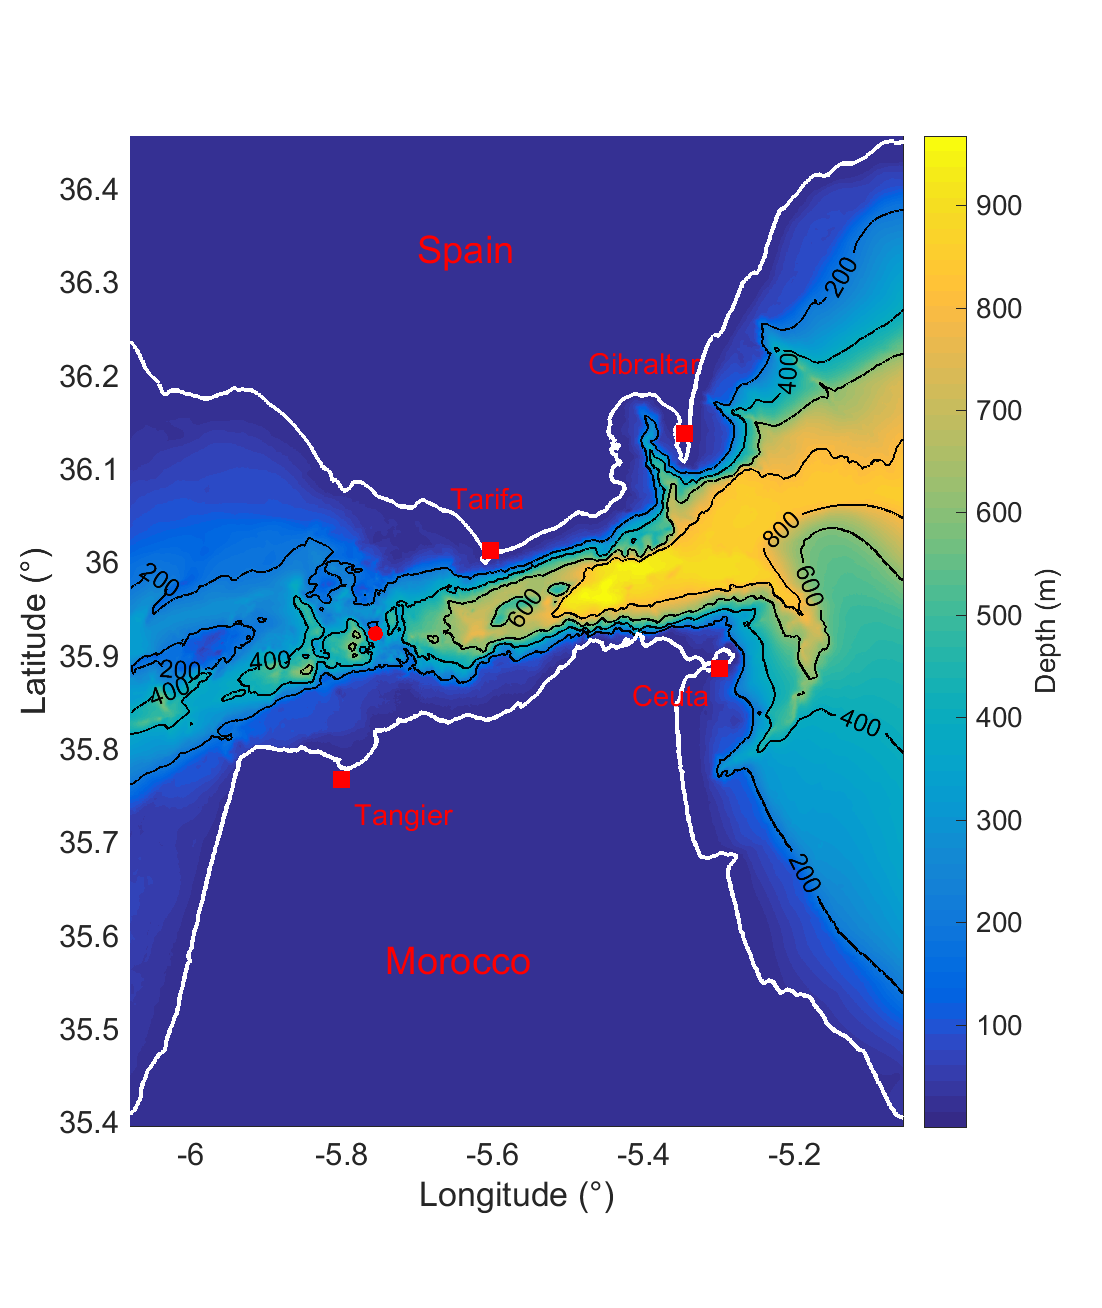
\includegraphics[width=0.5\textwidth]{./GBR3D/FigBathyVHR.png}
        \caption{Area and Bathymetry used for the simulations. The red dot denotes the point at Camarinal Sill where the zonal barotropic current is taken as reference in following figures.}
        \label{FigBathy3D}
\end{figure}

\begin{figure}[!h]
        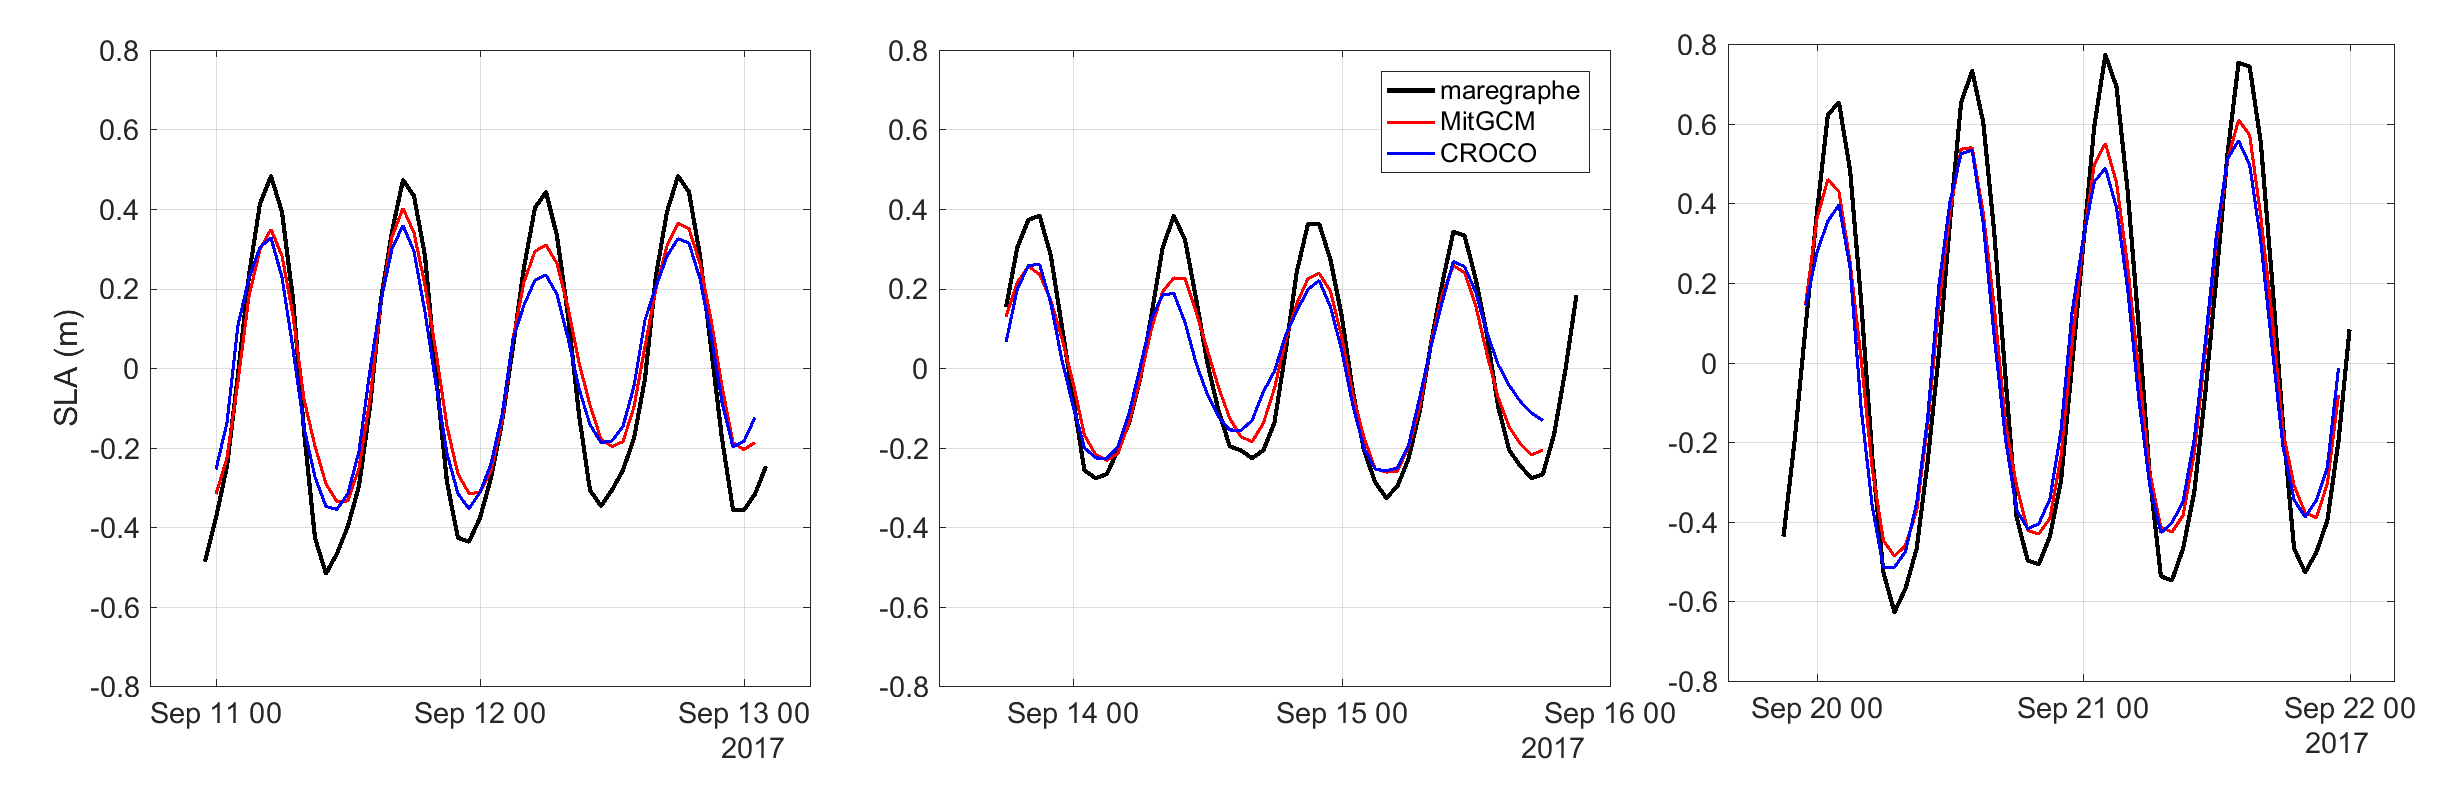
\includegraphics[width=\textwidth]{./GBR3D/SLA_Tarifa_ME2VE2IES.png}
        \caption{Sea level-anomaly at Tarifa: tidal gauge data (black), nearest grid point for parent MitGCM simulation (red) and CROCO simulation (blue) during ME (a), MM (b) and VE (c) events.}
        \label{fig_maree_tar}
\end{figure}

\subsubsection{Water masses.}
\label{sectionWaterMasses}
Figure (\noparref{Fig_Ini_WM3D}.A) and (B) show the $\theta-S$ diagrams in the eastern and western parts of the domain computed for the field of tracers used to initialize the simulation SimIT. 

\begin{figure}[!h]
        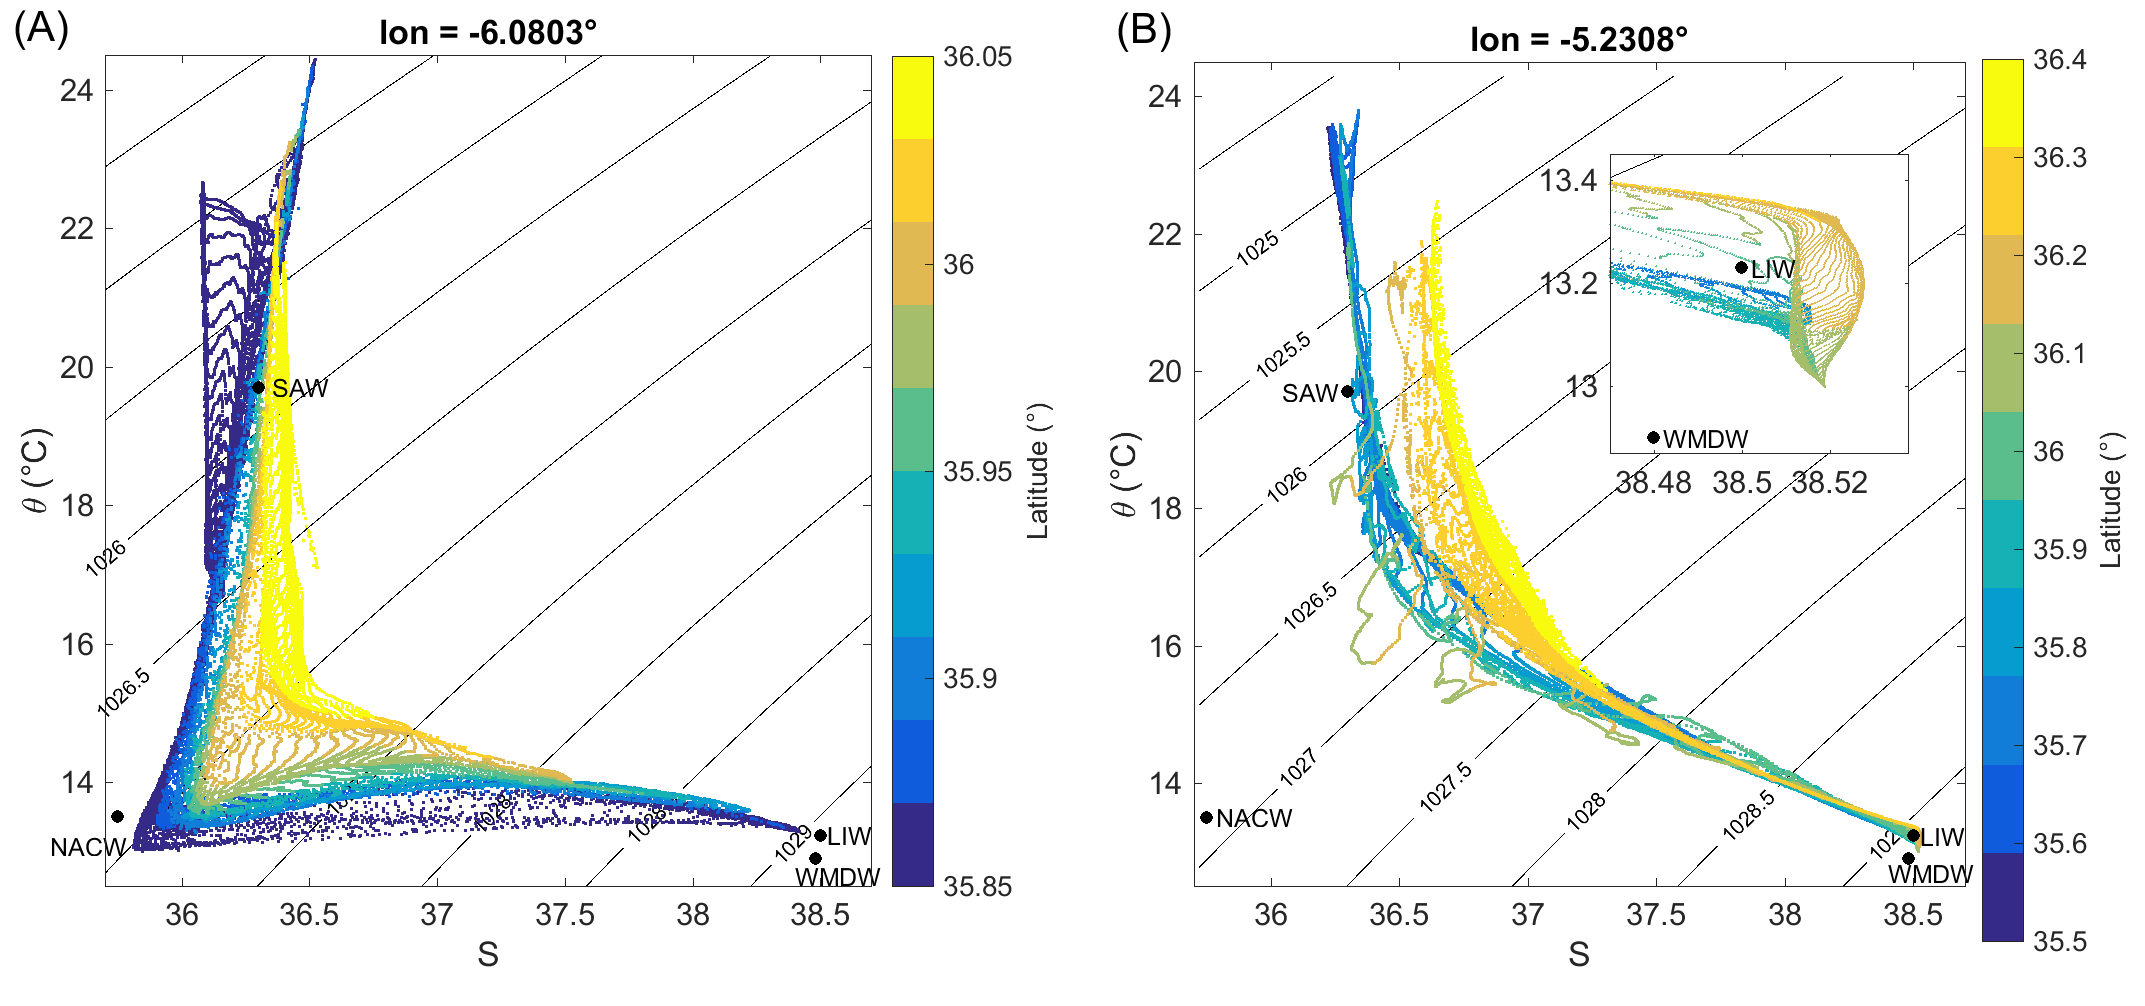
\includegraphics[width=\textwidth]{./GBR3D/WM_ini_IES.png}
        \caption{$\theta$-S diagrams computed at 6.08$^\text{o}$ W (a) and 5.23$^\text{o}$ W at first time step of SimIT. Color indicates the latitude of each grid point. Definition of the water masses according to \citet{naranjo_2014} are also indicated.}
        \label{Fig_Ini_WM3D}
\end{figure}

At the eastern boundary (figure (\noparref{Fig_Ini_WM3D}.B)), the signatures of a deep water mass and of an intermediate water mass that correspond respectively to WMDW and LIW can be identified. The latter is present mostly in the northern part of the domain. The simulated waters are however saltier and warmer than the corresponding water masses observed in the region as per \citet{naranjo_2014}.

At the western boundary now, the signature of two Mediterranean water masses corresponding to the two pathways of the Mediterranean outflow, centered around 35.8°North and 35.9°North, can be identified.
As far as Atlantic waters are concerned, NACW are mostly present on the western part of the domain. Its signal is minimized in the east of the domain, where surface waters are seen in figure (\noparref{Fig_Ini_WM3D}.B) to be saltier and colder over 36.2°N than at other latitudes.


%----------------------------------------------------------------------
\subsection{Numerical diagnosis}
%----------------------------------------------------------------------
\label{PartDiag3D}

\subsubsection{Hydraulic control}
\label{sectiondiagControl}

%\color{blue}The presence of an hydraulic control is probably the most important diagnostic to be carried out in the region of the Gibraltar strait. The exchange flow through the strait can shift from a so-called subcritical to a critical regime in only a few hours. This shift is associated to the occurrence (or not) of an hydraulic jump somewhere in the region of the strait. The bathymetry of the region is characterized by a complex network of pathways for the water masses which implies that hydraulic jump can appear or disappear locally. A consequence is that the classification of the whole strait in one "asymptotic" regime or the other is far from simple and probably not even necessary to explore the dynamics of the region.\color{red}(bof, laisser de côté...fait un peu introduction)

The flow in the Strait of Gibraltar can shift from subcritical to supercritical in only a few hours. Diagnosing the hydraulic state of theflow at each instant of the tidal cycle is then a necessity, and must be done locally to account to the complex bathymetry of the region. The effect of the complex bathymetry of the region, that makes such variations local, must also be taken into account. The definition of an instantaneous and local internal Froude number was already presented in chapter \ref{chapGBR2D} (see appendix \ref{app_Froude}), and is here refined not as a Froude number for the flow at a pecular grid point but to characterise either the flow of the atlantic or Mediterranean layer in the water column at a given coordinate.

%\color{black}

%((Diagnostics carried out in the 2D, academic configuration proposed in section {XXX} consequently need to be refined and, in any case, must be local.\\

%To start with, "a" local Froude number needs to be computed and,\color{red}meeeehh\color{black}
To do so,  the superposition of the Atlantic and Mediterranean water masses (when effective) is chosen as a simple two-layer (at most three-layer if one wants to single the interface) representation of the stratification.

In the previous section \ref{sectionWaterMasses}, Atlantic and Mediterranean water masses have been clearly identified based on their signature in temperature and salinity. Salinity is probably the most pertinent tracer to differentiate these waters in the region of the strait due to the large contrast of salinity existing between Mediterranean and Atlantic water masses.
An approximate, local, two-layer analysis can thus be carried in the present, fully-3D , realistic configuration if an interface is defined in regard to a reference salinity. In this case, its depth is defined as the height of the first water parcel \sout{from the top down} in the water column for which salinity is above the intreface reference salinity.

This reference salinity $S_i$ is taken as varying along the strait as a hyperbolic tangent function of longitude centered at CS to account for the different water mass composition in the eastern and western part of the Strait of Gibraltar. 

\begin{equation}
	S_i(l)=tanh(\frac{l-L_{CS}}{dl})\frac{S_M-S_m}{2}+\frac{S_M+S_m}{2}
	\label{eqSinterface}
\end{equation}
with $L_{CS}=5.75^o$, $dl=0.25^o$, the location and width of the Camarinal Sill in degrees, $S_M=37.39$ and $S_m=37.1$ the max and minimum interface values taken respectively east and west of the sill.

With the Atlantic and Mediterranean layers defined above, the Froude layer number for internal gravity waves is computed for a given water column as: 

\begin{equation}
F_i=\frac{U_i^2}{g'h_i} , \ \text{with} g'=g \ \frac{\rho_2-\rho_1}{\rho_0}
\end{equation}
where $\rho_i$ is the averaged density, and  $U_i$ the averaged velocity norm, over the layer $i$ of height $h_i$. $F_i>1$ means that the flow in layer $i$ is supercritical.


\subsubsection{Hydraulic jump detection, acceleration of flow}
\label{sectiondiagJump}
However, the necessity to caricature the stratification, but also to evaluate a local phase velocity of internal waves based on this stratification, renders the evaluation of a local Froude number rather complex and, as a consequence, can somehow blur the characterization of the local regime of the dynamics. One process that needs to be properly evaluated is the presence of the hydraulic jump over Camarinal Sill, a feature of the flow that has a role in both the generation of ISWs and in local mixing of the water masses.


A simple diagnosis for the detection of the hydraulic jump at Camarinal Sill in the simulations is proposed based on the impact such a structure is known to have on the flow. 
\begin{figure}[!h]
 \centering
 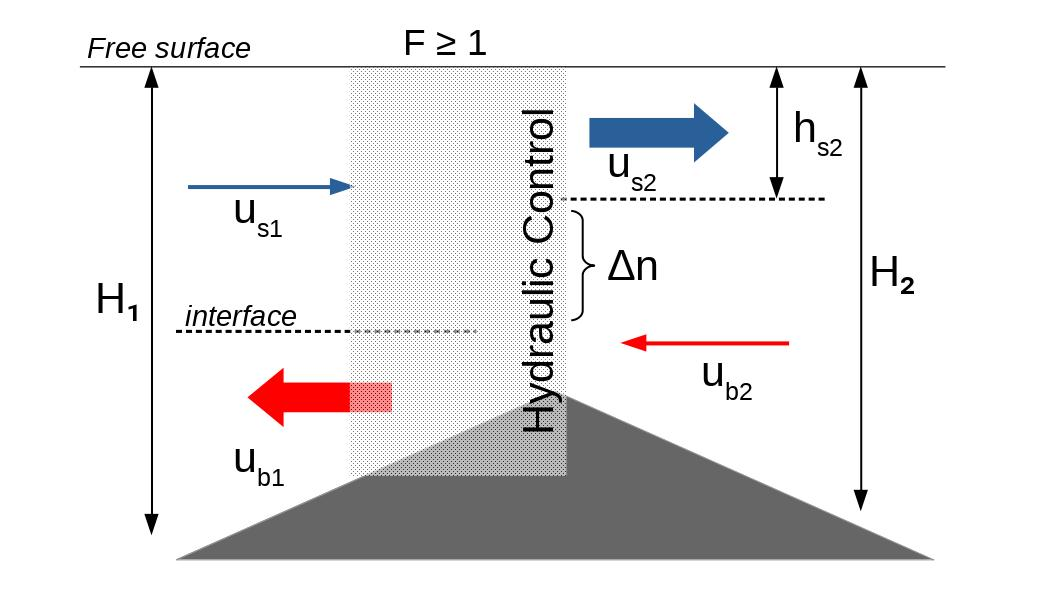
\includegraphics[width=0.5\textwidth]{./GBR3D/schema_diagressaut.jpg}
 \caption {Schematic of flow upstrean and downstream of hydraulic jump at Camarinal Sill in the Strait of Gibraltar.}
  \label{schemaRH}
\end{figure}
As schematized on figure \ref{schemaRH}, an hydraulic jump (also called hydraulic drop) induces a drop of the interface depth. Since the flow in the Strait is channeled by the bathymetry (for the Mediterranean flow at least) and the coast (for the Atlantic flow), there must be conservation of the flux from a downstream section to an upstream section of the hydraulic jump. The variation of the interface depth is indeed associated to an acceleration or a deceleration of the flow (depending on which layer is chosen as a reference).
%\color{green}Je pense qu'il faut changer les notations et conserver plutôt $h_*$ pour les épaisseurs plutôt que b, notation souvent utilisée pour la flottabilité et n pour une numération entière." \color{black}
The drop in the interface depth is noted $\Delta n=h_{s2}-h_{s1}$, the variation of bottom depth $\Delta H=H_2-H_1$ and the acceleration in the bottom layer $\Delta u_b = u_{b2}-u_{b1}$. In the bottom layer, the conservation of the flux leads to:
\begin{subequations}
\begin{alignat}{2}
  \displaystyle
&u_{b1} (H_1-h_{s1})&& = u_{b2} (H_2-h_{s2})\\
& &&= u_{b1} (\Delta H + \Delta n) + u_{b1} (H_1-b_1) + \Delta u_b (H_2-h_{s2})
\end{alignat}
\end{subequations}

\begin{equation}
\Delta u_b = -u_{b1} \frac{\Delta H + \Delta n}{H_2-h_{s2}}
\end{equation}

For the surface flow:
\begin{equation}
\Delta u_s = - u_{s1}\frac{\Delta n}{h_{s2}}
\end{equation}

The velocity in the area of the hydraulic jump must validate the condition of (at least) critical flow, i.e. Froude number $\geq$ 1 at the shallower location. A minimal condition for hydraulic jump is consequently  $U\ =\ c$ ($F\ =\ 1$) : the flow velocity must be equal to the local phase speed of internal waves. An expression for $u_{b,s1}$ is given by the definition of interfacial velocity : 
\begin{equation}
|u_1|=c=\sqrt{g' \frac{(H_1-\Delta n - h_{s2})(\Delta n + h_{s2})}{H_1}}
\end{equation}
 %\color{green}Il faut que tu reformules et que tu expliques un peu plus ce qui suit... difficilement reproductible par un lecteur qui découvre ce diagnostique. Tu peux ajouter une petite explication en annexe si tu as peur que cela fasse trop dans la partie principale. \color{black} 
In this formulation, $H_1$,$H_2$ and$\Delta H$ are the local depths of the water column at anay coordinate. $\Delta n$, $h_{s2}$ and $g'$ are \textit{a priori} unknown.

But the values of $\Delta u_b$ and $\Delta u_s$ are used as theoretical threshold to be compared to the actual variation of the flow between two grid points in the model. This treshold only needs to be chosen as small enough that greater increase of the flow velocity can be attributed to an hydraulic jump, and the set of parameters ($\Delta n$, $h_{s2}$, $g'$) are chosen empirically here as the vertical excursion of the interface $\Delta n = 30m$, the depth of the Atlantic layer $h_{s2}=50 m$ , and the reduced gravity $g'\ =0.02\ m.s^{-2}$.

\subsubsection{Q parameter and derivated diagnosis}
\label{sectiondiagQ}

The studied configurations are all based on grid resolutions of a few tenths of meters, an objective being the explicit simulation of at least the largest turbulent eddies. The region of the Mediterranean outflow is of particular interest since large velocity shears are known to be associated there to a large vertical density (salinity) stratification, and may overcome this stratification's stabilizing effect to give rise to the devlopment of shear instabilities. %This region is thus a key area to better understand and simulate the mixing of Mediterranean and Atlantic water masses in Gibraltar strait.

A dedicated diagnostic is now proposed to "detect" primary instabilities and more specifically to identify Kelvin-Helmholtz instabilities potentially developing in this region. 
A careful inspection of the relative-vorticity vector can fulfill this purpose and a dedicated scalar diagnostic based on the components of this relative vorticity is retained. It is a generalization of the Okubo-Weiss parameter retained in Hilt (2020) (chapter \ref{chapGBR2D}, see appendix \ref{annexeOW}) to the present 3D realistic configurations. 
%A simple vorticity diagnosis is not chosen as it requires choosing the rotation axis, but also because regions of high shear such as between the MEd outflow and Atl waters will have high vorticity values. Instead, analogously to the use of the Okubo-Weiss parameter in Hilt 2020, we chose to compute parameter Q, defined as (ref):
\begin{equation}
Q=-\frac{1}{2} \frac{\partial u_i}{\partial x_j} \frac{\partial u_j}{\partial x_i} = \frac{1}{2} (\Omega_{ij}\Omega_{ij} - S_{ij} S_{ij})
\end{equation}
with $u_i$ the components of velocity vector, and $S_{ij}$ and $\Omega_{ij}$ are respectively the strain-rate tensor and vorticity tensor. When $Q\ >\ 0$, rotation is larger than shear.
%\color{green}Attention à la cohérence des notations ui etc... tout au long du manuscrit. $\Omega$ est en particulier déjà utilisé pour la rotation de la terre, $\omega$ est plus courant pour la vorticité relative.\color{black}

Statistical description of the field of this parameter $Q$ are carried out in the following sections. In particular, the standard deviation of parameter $Q$ is :
\begin{equation} 
\label{eqstdQ} 
    std ( Q ) (\mathbf{x},\ t)=  \sqrt{   \overline{Q (\mathbf{x},\ t)^{2}} -  \overline{Q(\mathbf{x},\ t)}^{2}  }
\end{equation}
where the overbar denotes an average over 30 minutes, a time-scale considered here as smaller than the time-scales of the fine-scale dynamical structures the present study is interested in, but over which the variations of the large-scale flow are not too important.

This description is compared to Singular Value Decomposition (SVD) presented in annexe \ref{annexeSVD}. SVD computations requires a priori the storage of the field to be decomposed. Contrary to the computation of the standard deviation of $Q$, this could not be made online and SVD have consequently been computed off-line. This necessitates high frequency 3D outputs to pick up the relevant structures, so for storage space reason SVD could only be carried out on limited areas.  


%----------------------------------------------------------------------
\subsection{Fine scales in the strait of Gilbraltar}
%----------------------------------------------------------------------
\label{section3DRes}

\subsubsection{Hydraulically controlled layer and hydraulic jumps, neap-spring tide variability}
\label{section3DResFlow}

\begin{figure}[!h]
 \centering
 
 \begin{subfigure}{\linewidth}
\centering
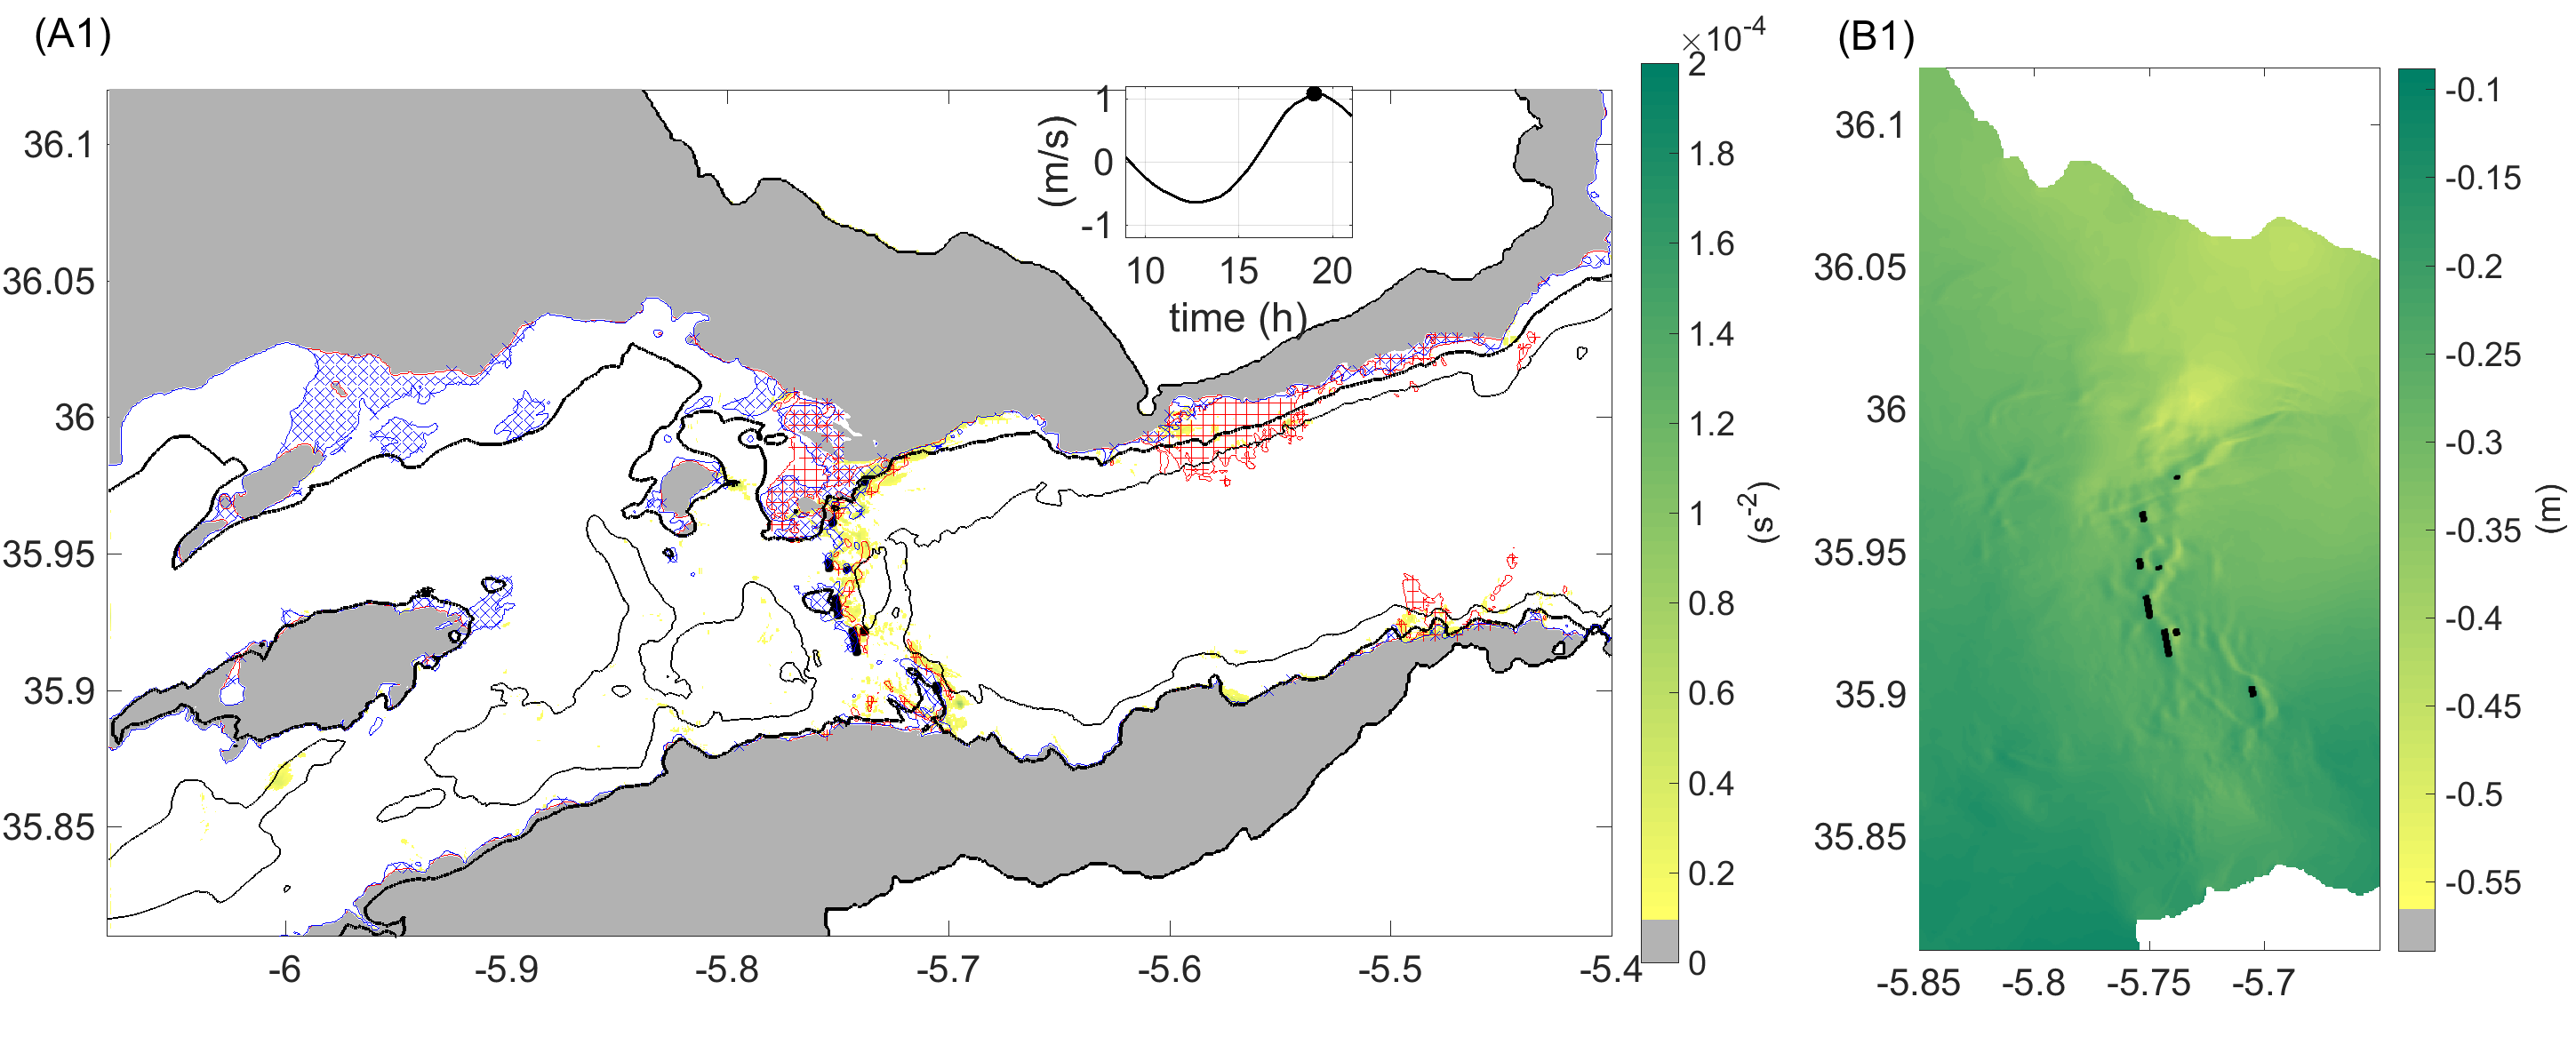
\includegraphics[width=1\linewidth]{./GBR3D/ME2_19h_p.png}
\end{subfigure}
 
 \begin{subfigure}{\linewidth}
\centering
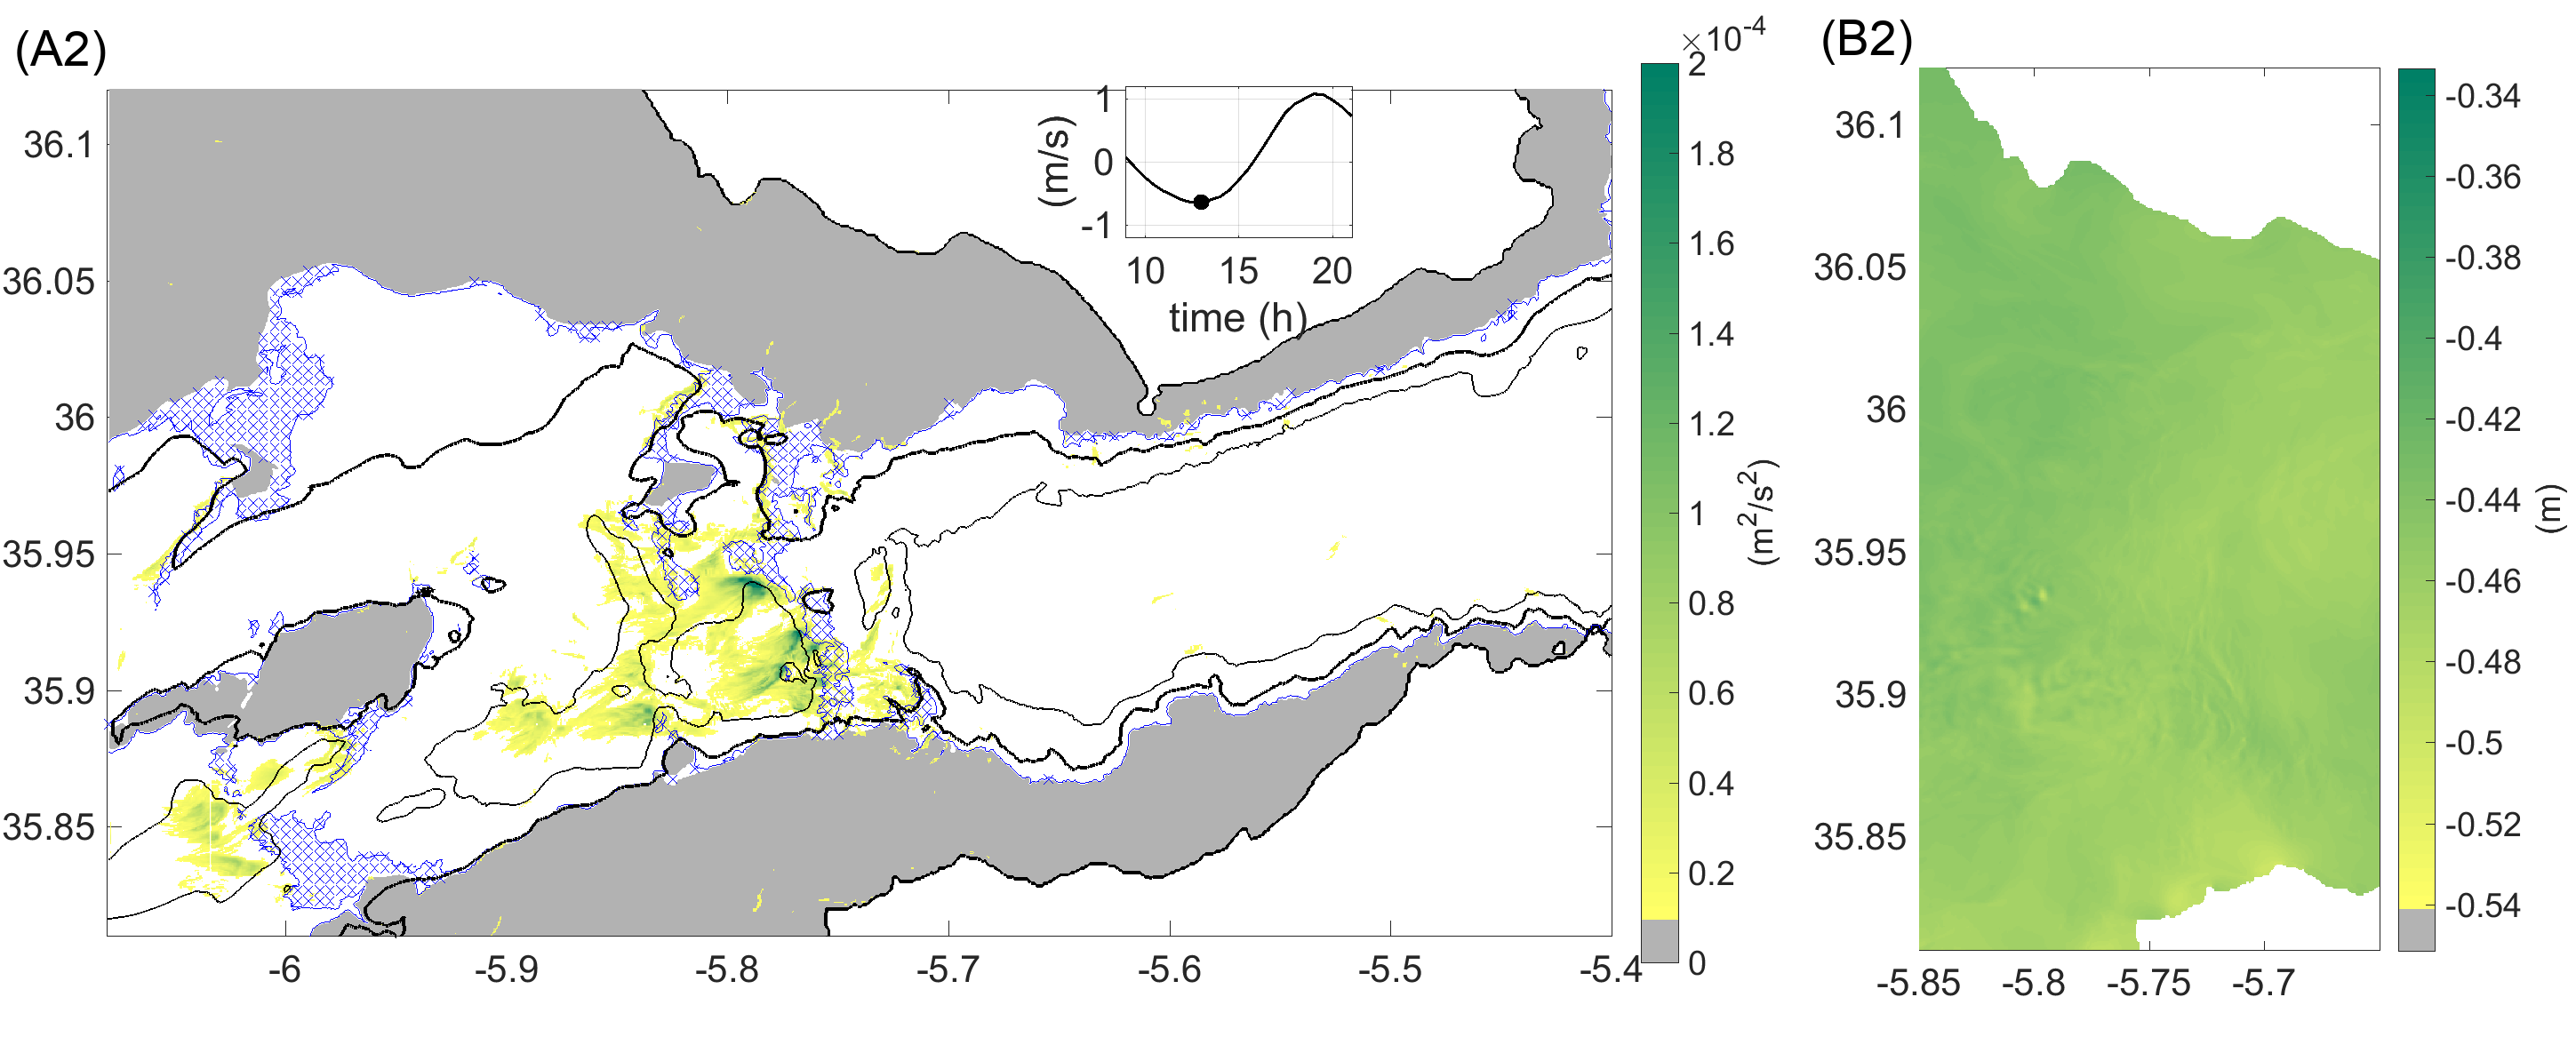
\includegraphics[width=\linewidth]{./GBR3D/ME2_13h_p.png}
\end{subfigure}
\caption { (A1 and A2) Consecutive inflow and outflow in configuration SimNT, \textit{no-jump} case. The blue (red) shaded areas correspond to supercritical Mediterranean (Atlantic) layers (\S \ref{sectiondiagControl}). Black dots show locations where an hydraulic jump has been detected (\S \ref{sectiondiagJump}). The grey areas denote where $S_{bottom}\ <\ S_{interface}$, the salinity in the bottom grid point is lesser than the interface salinity defined in section\ref{sectiondiagControl}. Colorbar is related to the standard deviation of parameter Q (section \ref{sectiondiagQ}, only values above $10^{-5} s^{-2}$ are represented). Barotropic zonal currents at CS (point indicated in figure \ref{FigBathy3D} are also indicated). Two black isobathes contours are shown: 200 m (bold) and 400 m (thin). (B1 and B2) field of sea level anomaly in the areo of CS and black dots indicating detection of an hydraulic jump as in (A1 and A2).}
\label{FigHCN}
\end{figure}

Figures \ref{FigHCN} to \ref{FigHCI} present several diagnosis for a series of maximal outflows and inflows with variable strength of the tidal forcing in configurations SimNT, SimST and then SimIT (tables \ref{tab_sim3Dnames} and \ref{tab_dates_MIV}). The corresponding diagnosis are presented in paragraph \ref{PartDiag3D}: the shaded regions correspond to areas of supercritical flows (\S \ref{sectiondiagControl}) in either the Atlantic (red) or Mediterranean(blue) layers. On top of these shaded regions, the locations of hydraulic jumps are indicated (\S \ref{sectiondiagControl}) together with the areas of large standard deviations of parameter Q (\S \ref{sectiondiagQ}) (the latter is discussed in section \ref{sectionsim3D_res_insta}) The grey area indicates where the salinity in the bottom level is below the interfacial salinity as defined in equation \ref{eqSinterface}, and thus where Atlantic waters are exclusively present in the water column. 

Figure \ref{FigHCN} presents a neap-tide situation of weak barotropic currents ($\ <\ 1\ m/s$ at a shallow point of CS) in both outflow and inflow conditions. Figure \ref{FigHCS} corresponds to strong barotropic currents ($\geq 1.5\ m/s$) in inflow and outflow conditions during a spring-tide period. Finally, figure \ref{FigHCI} corresponds to a period of outflow with intermediate-strength ($\approx 1\ m/s$) of the barotropic currents.

\begin{figure}[!h]
 \centering
\begin{subfigure}{\linewidth}
\centering
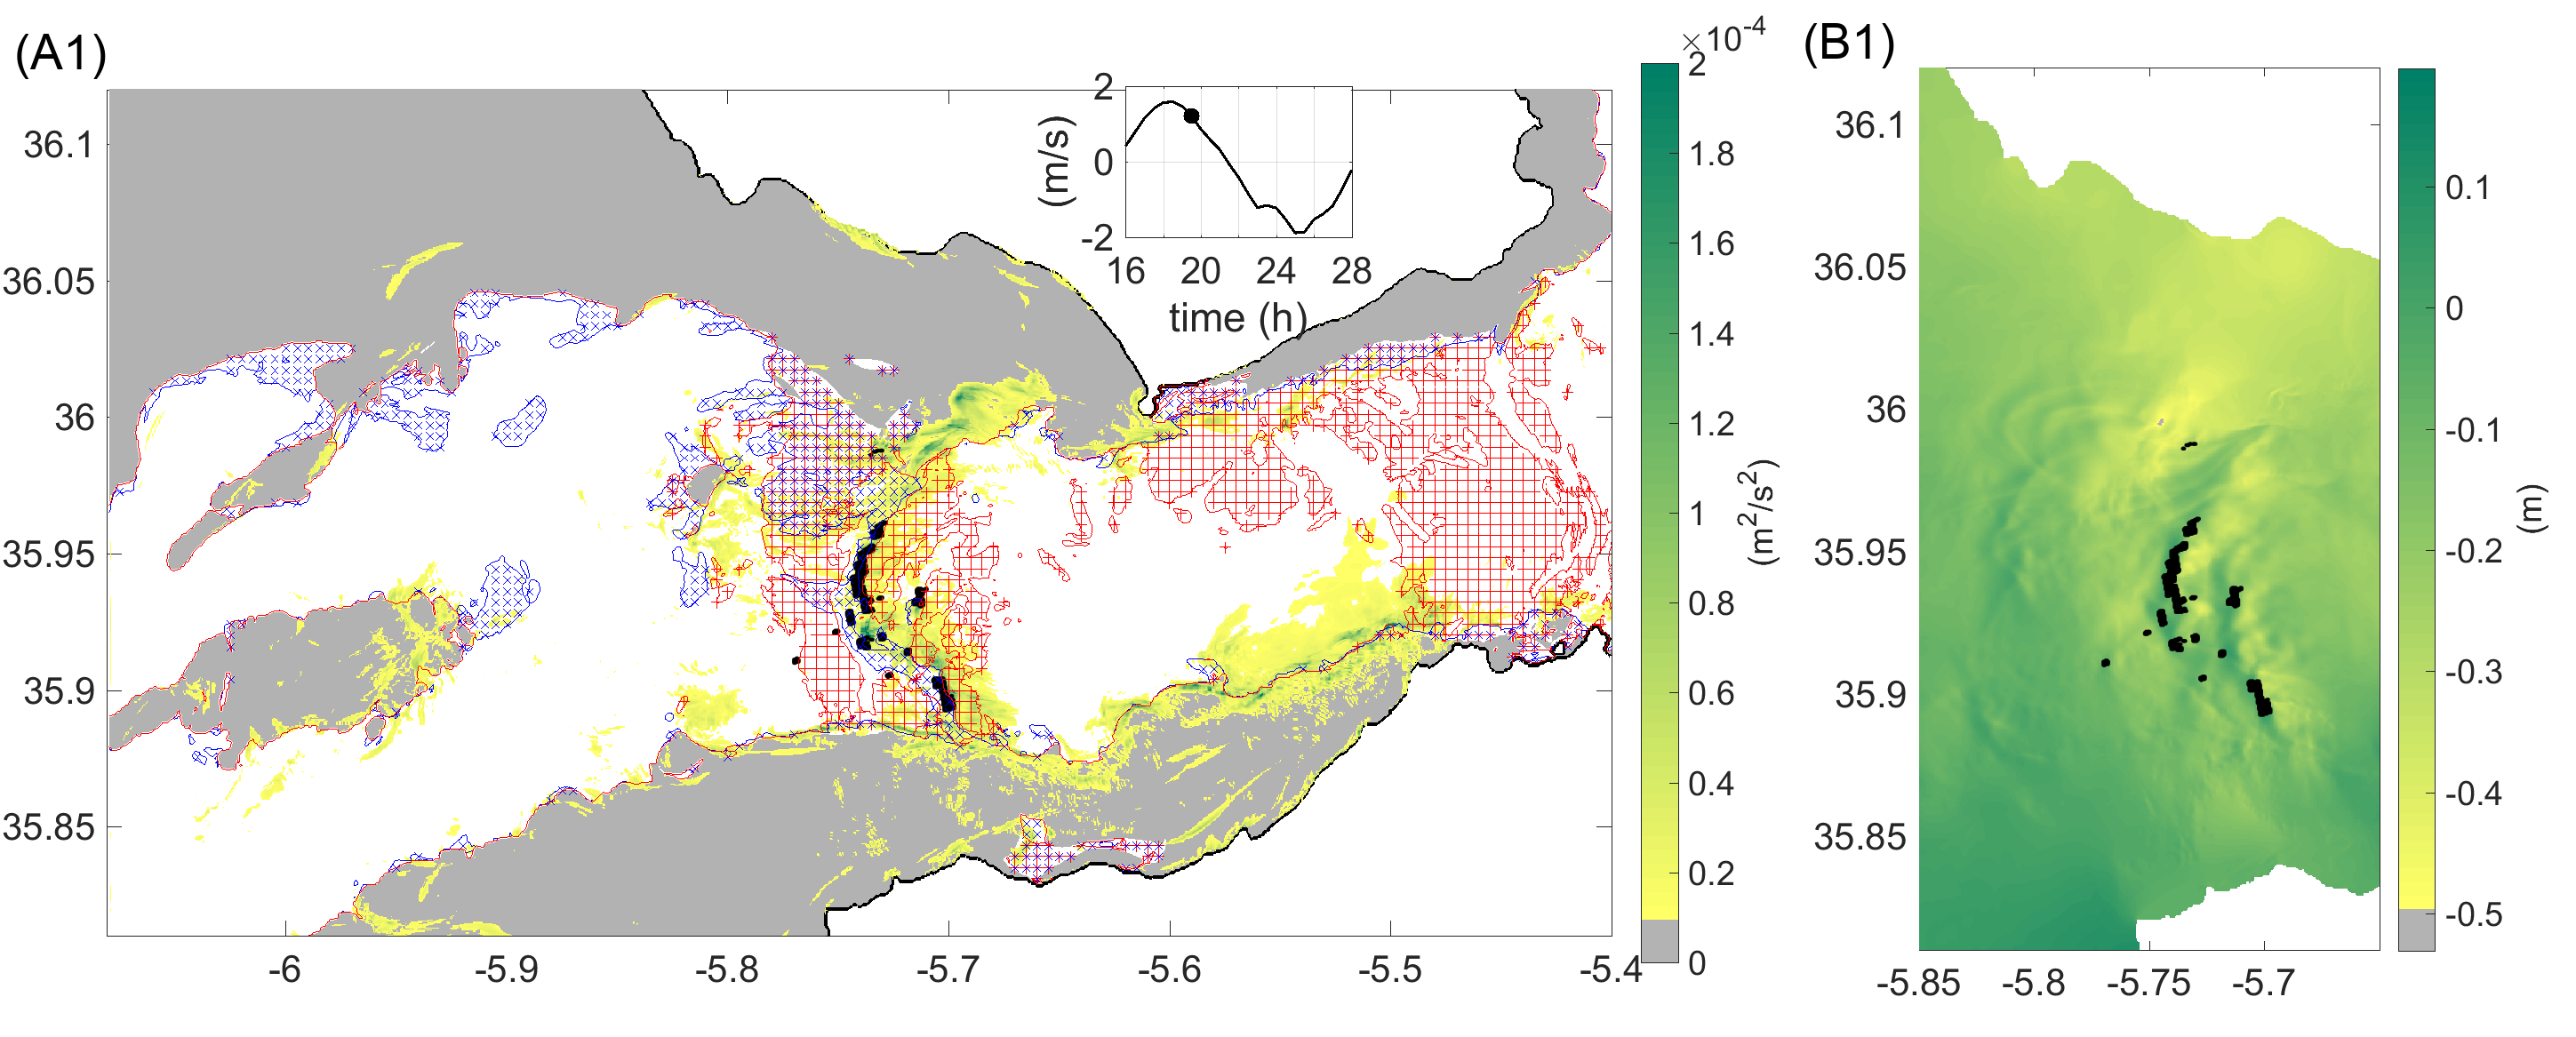
\includegraphics[width=\linewidth]{./GBR3D/VE2_19h30_p.png}
\end{subfigure}

\begin{subfigure}{\linewidth}
\centering
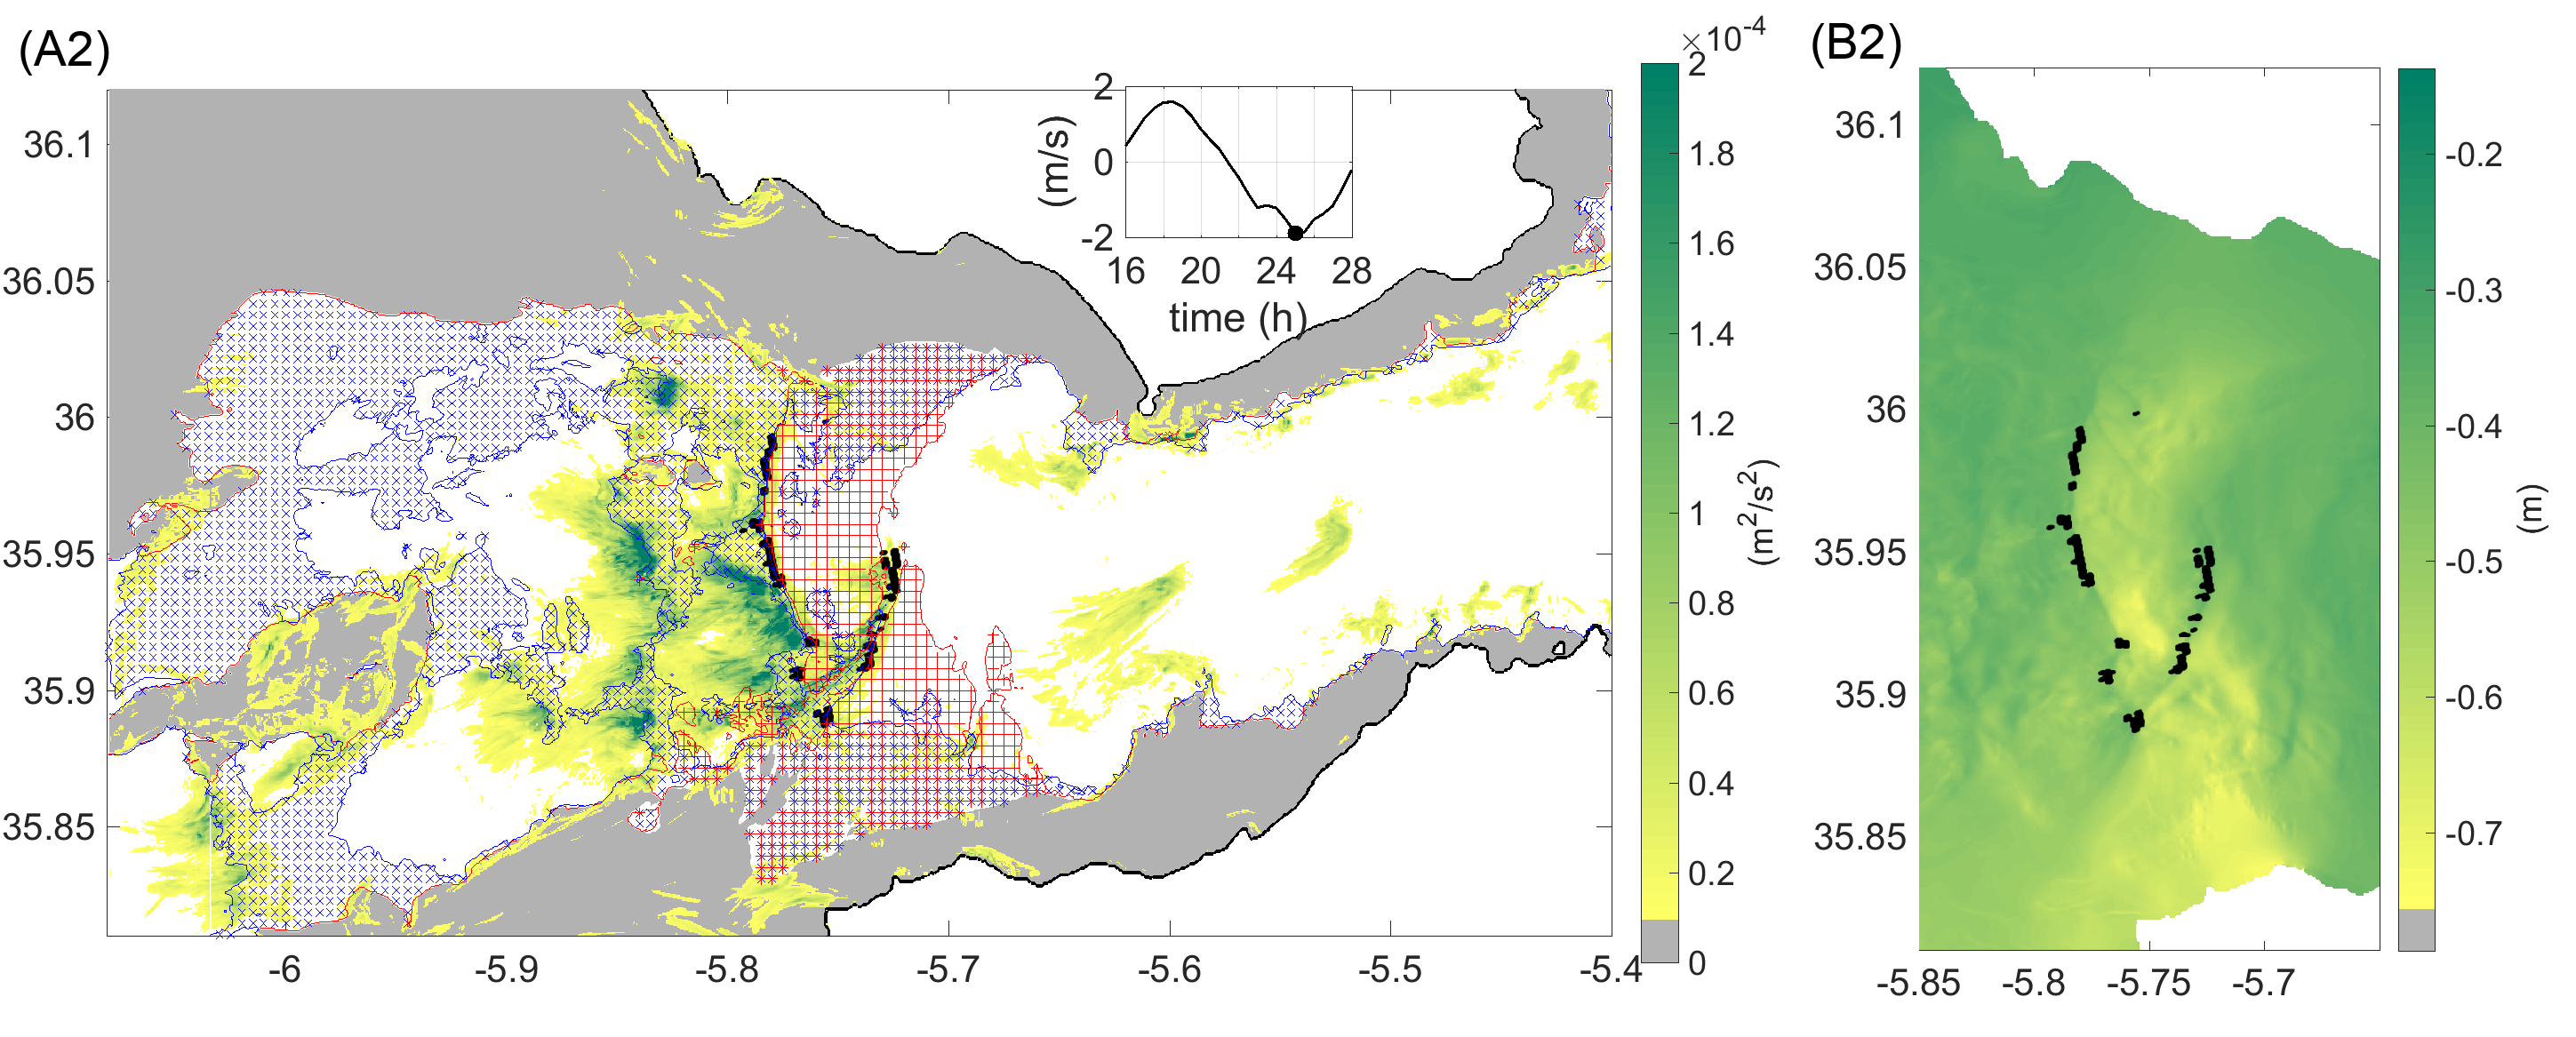
\includegraphics[width=\linewidth]{./GBR3D/VE2_25h_p.png}
\end{subfigure}
\caption {Same as figure \ref{FigHCN} but for simulation SimST in inflow and outflow of type \textit{w-jump}}
\label{FigHCS}
\end{figure}

\begin{figure}[!h]
 \centering
%\begin{subfigure}{\linewidth}
%\centering
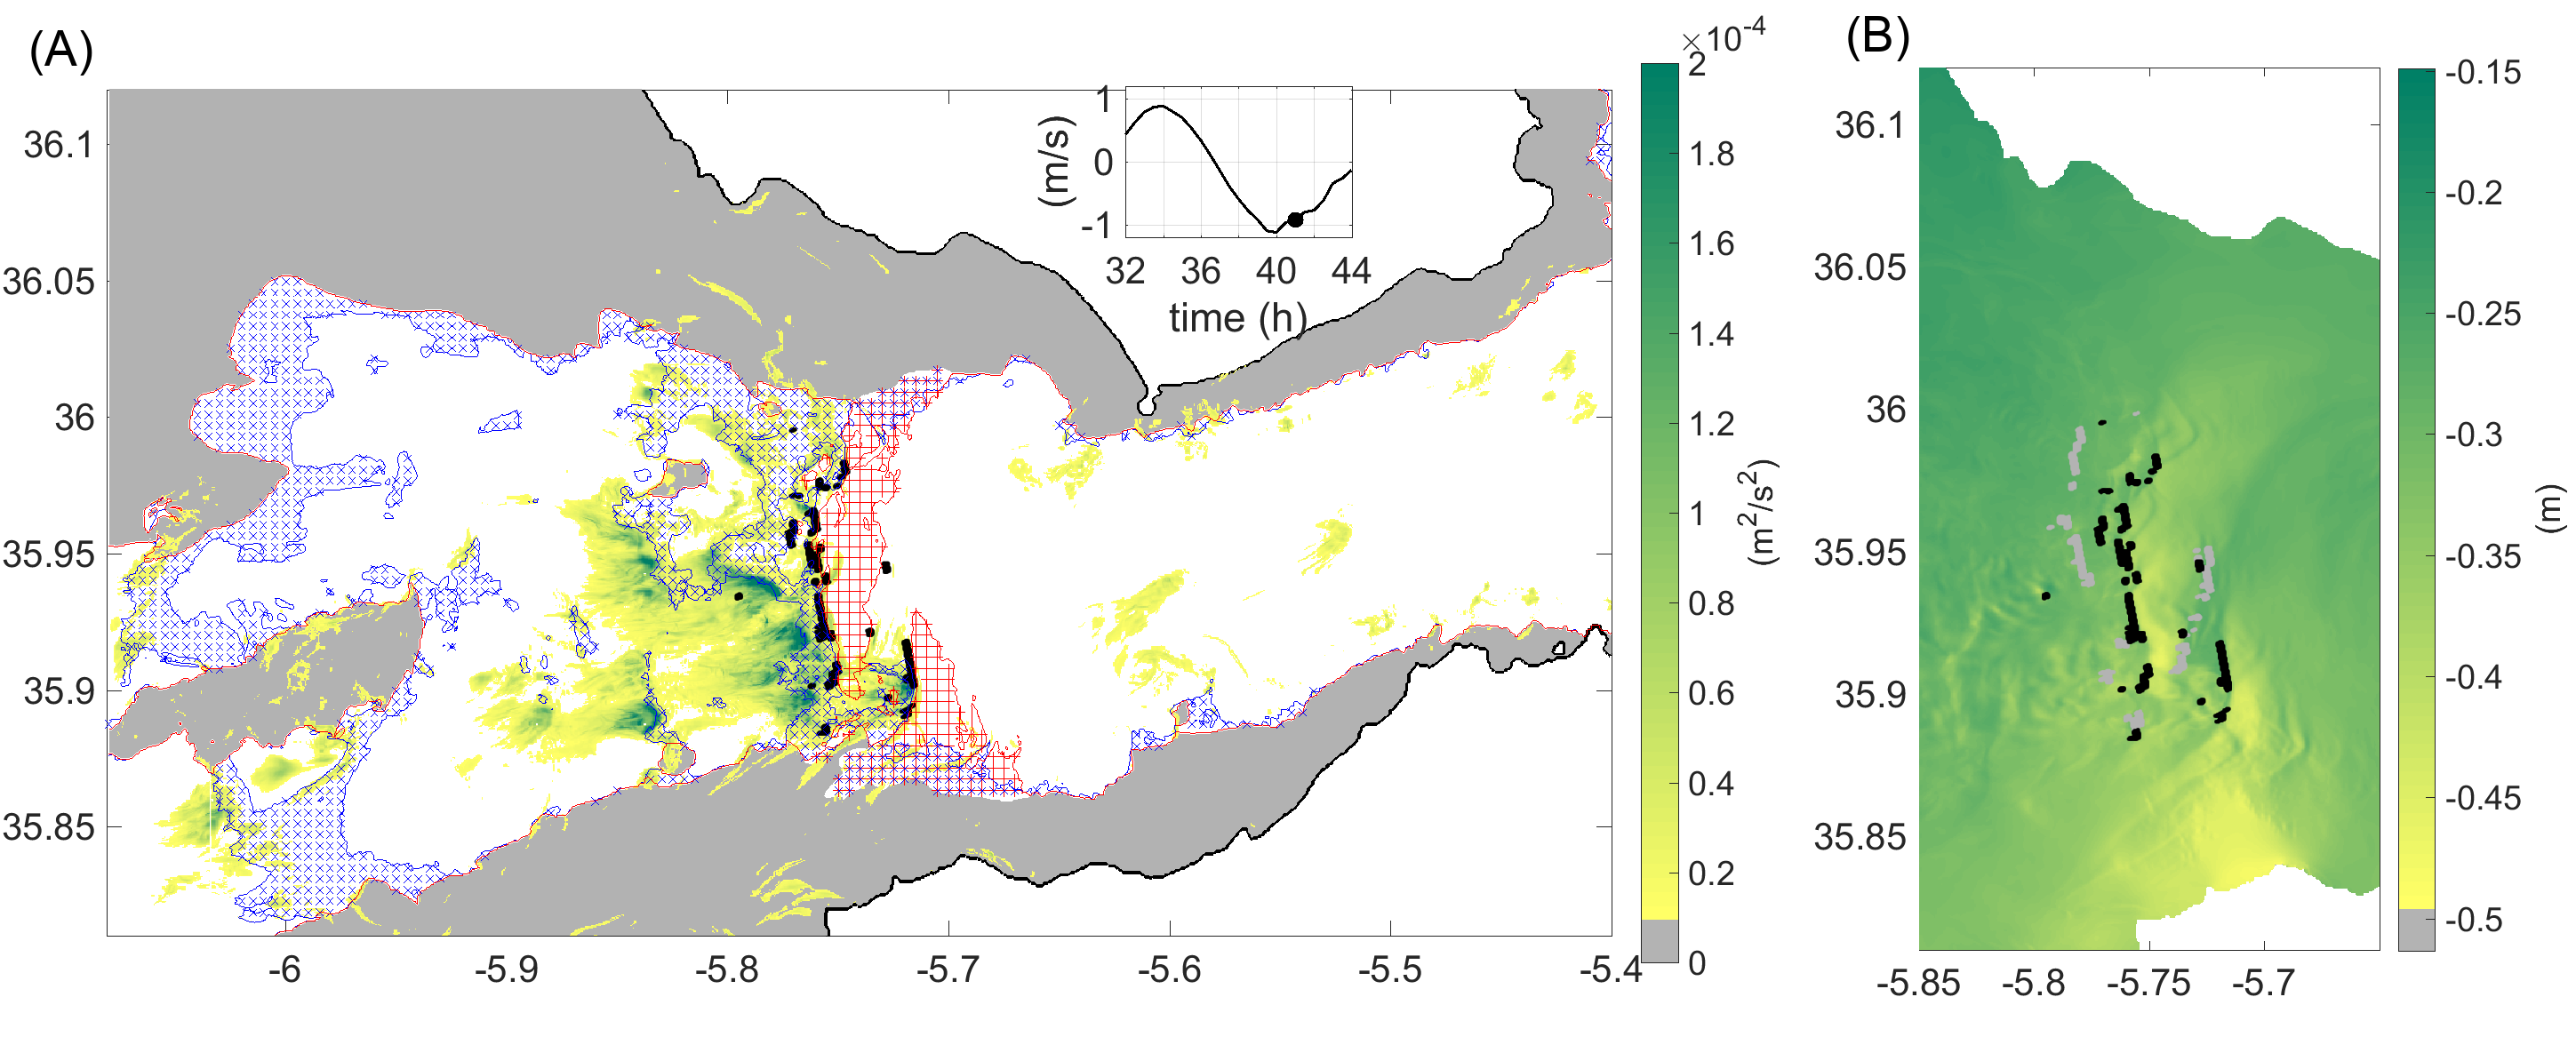
\includegraphics[width=\linewidth]{./GBR3D/IES_41h_p.png}
%\end{subfigure}
 \caption {Same as figure  \ref{FigHCN} but for simulation SimIT and an outflow of type {s-jump}. The sea surface anomaly (SLA) shows the signature of the hydraulic jump of spring tide outflow}
 \label{FigHCI}
\end{figure}

%\color{green}Attention, tu as laissé beaucoup de formulations sans verbe de ce type: 
%\sout{Firstly, can see two channels west of the Camarinal Sill where Med layer is present, separated by Majuan Bank.} ???\color{black}
Firstly, two veins of Mediterranean water separated by Majuan are systematically found west of CS in figure \ref{FigHCN} to \ref{FigHCI}.
 %\sout{The southern vein does not change much, however in the northern channel see a variable area of circulation for med waters above 200m depth and centered at 36$^\text{o}$ N.} \color{green}Reformule lorsque pas de sujet... la tournure me semble peu usuelle en anglais ? Une proposition suit:\\
 %\color{blue}
The southern vein does not change much accross situations. In the northern channel, however, an area of possible circulation of the Mediterranean outflow (non-grey area) roughly centered at 36°N;5.95°W with bottom depth of 200m is seen as variable. This area is larger during outflows (compare for exemple figures (\noparref{FigHCS}.A1) and (A2)), as Mediterranean waters are driven up-slope by the westward barotropic current. But the flow presents an additional southern component that bends back into the deeper main northern channel (see figure \ref{FigBathy3D} for a better view of the bathymetry of this area).

For all cases, supercritical areas of the Atlantic (Mediterranean) layer can be found mostly east (west) of 5.8 $^\text{o}$ W which corresponds to the western slope of CS. During inflows in figure (\noparref{FigHCN}.A1) and (\noparref{FigHCS}.A1), the Mediterranean layer becomes supercritical over several regions (patches are observed): the most extended one in the area of the northern channel has been discussed above. In outflows in Figures (\noparref{FigHCN}.A2), (\noparref{FigHCS}.A2) and (\noparref{FigHCI}.A), the Mediterranean layer is supercritical at both Camarinal and Espartel sills and in the northern channel.  During the spring tide outflow period, most of the northern channel presents a supercritical flow while over ES, there is not much difference between the intermediate and spring tide outflow periods.

Foa all outflow cases, the Atlantic layer is supercritical only at CS, except during the neap tide period (see figure (\noparref{FigHCN}.A2)) when it isn't supercritical anywhere. In cases where both the Mediterranean and Atlantic layers are supercritical at CS, an hydraulic jump is detected. It is located at the intersection of areas where Atlantic and Mediterranean layers are supercritical. This configuration leads to an area of high gradients of free-surface elevation (figures (\noparref{FigHCS}.B2) and (\noparref{FigHCI}.B)). For both of thoses outflow cases, two hydraulic controls are detected in the area of Camarinal Sill, a western one (west of 5.75°W in figure (\noparref{FigHCI}.B)) linked to the sill itself, and an eastern one (east of 5.725°W in figure (\noparref{FigHCI}.B)) linked to secondary bathymetric features.

Among the simulated tidal cycles, three types of flows can be encountered at CS for the outflow periods: (i) no hydraulic jump (\textit{no-jump}), (ii) the western hydraulic jump is located right above the sill (figure (\noparref{FigHCI}), \textit{s-jump}), and (iii) the western hydraulic jump is located over the western slope of CS (figure (\noparref{FigHCS}.A2) and (B2), \textit{w-jump}). In this latter case, the western hydraulic jump actually develops over the sill's crest as in the \textit{s-jump} case but since the tidal currents continue to strengthen, the area of supercritical Atlantic flow broadens. The junction between supercritical and critical flow is shifted west over the slope of the Sill where an hydraulic jump can be observed. The same evolution applied to the eastern hydraulic jump, see figure (\noparref{FigHCI}.B). 

An hydraulic jump also appears during inflows, it remains in the same area over the east slope of CS regardless of the strength of tidal currents. It is more well-defined when barotropic currents are stronger, compare figures (\noparref{FigHCN}.B1) and (\noparref{FigHCS}.B1).

East of CS, another area of supercritical Atlantic layer appears during inflows. During neap-tide (figure (\noparref{FigHCN}.A1)), it takes the appearance of a patch near the north shore in Tarifa Narrows at 5.59$^o$ W. During spring tide (figure (\noparref{FigHCS}.A1)), this patch extends over a larger area and a secondary area of supercritical Atlantic flow exists between 5.5$^o$ W and 5.4$^o$ W, extending from the northern to the southern side of Tarifa Narrows. 

Figure (\noparref{FigISWGBR3D}.A) and (B) shows the divergence of surface currents in Tarifa Narrows while a train of ISW is propagating there. In both figures, it is visible as an alternance of negative and positive surface currents divergence (when seen from west to east) between 5.4°W and 5.45°W. Figure (\noparref{FigISWGBR3D}.A) corresponds to a barotropic current of intermediate strength in SimIT during inflow and figure (\noparref{FigISWGBR3D}.B) to a strong barotropic current during the inflow of another tidal cycle in SimST (teh time is the same as in figure (\noparref{FigHCS}.A2)). The areas of critical Atlantic layer flow are also shown as a black meshed area. 

In figure (\noparref{FigISWGBR3D}.A), two distinct areas of supercritical Atlantic flow are located immediately west of the ISWs and in the northwest at 36°N, both as moderatly extended patches. Looking at figure (\noparref{FigHCN}.A1) the situation is similar for that inflow of SimNT. In figure (\noparref{FigISWGBR3D}.B), for which the barotropic currents are stronger, the first patch overlays half of the propagating train of ISWs and joins the northwestern patch, so that the flow of the whole Atlantic layer is supercritical at this moment and at all latitudes between 5.4°W and 5.45°W.

%It is located west of the propagating wave train. (je crois que je ne comprends pas où tu veux en venir?)\color{blue} The northern part of the critical area of the Atlantic layer seems to be dissociated from its southern part. The former occurs more often and its extension varies  \sout{while} whereas the latter may be modified by the arrival of the ISWs. This can be due either to the induced velocity or to the change of stratification.\color{black}

\begin{figure}[!h]
 \centering
%\begin{subfigure}{\linewidth}
%\centering
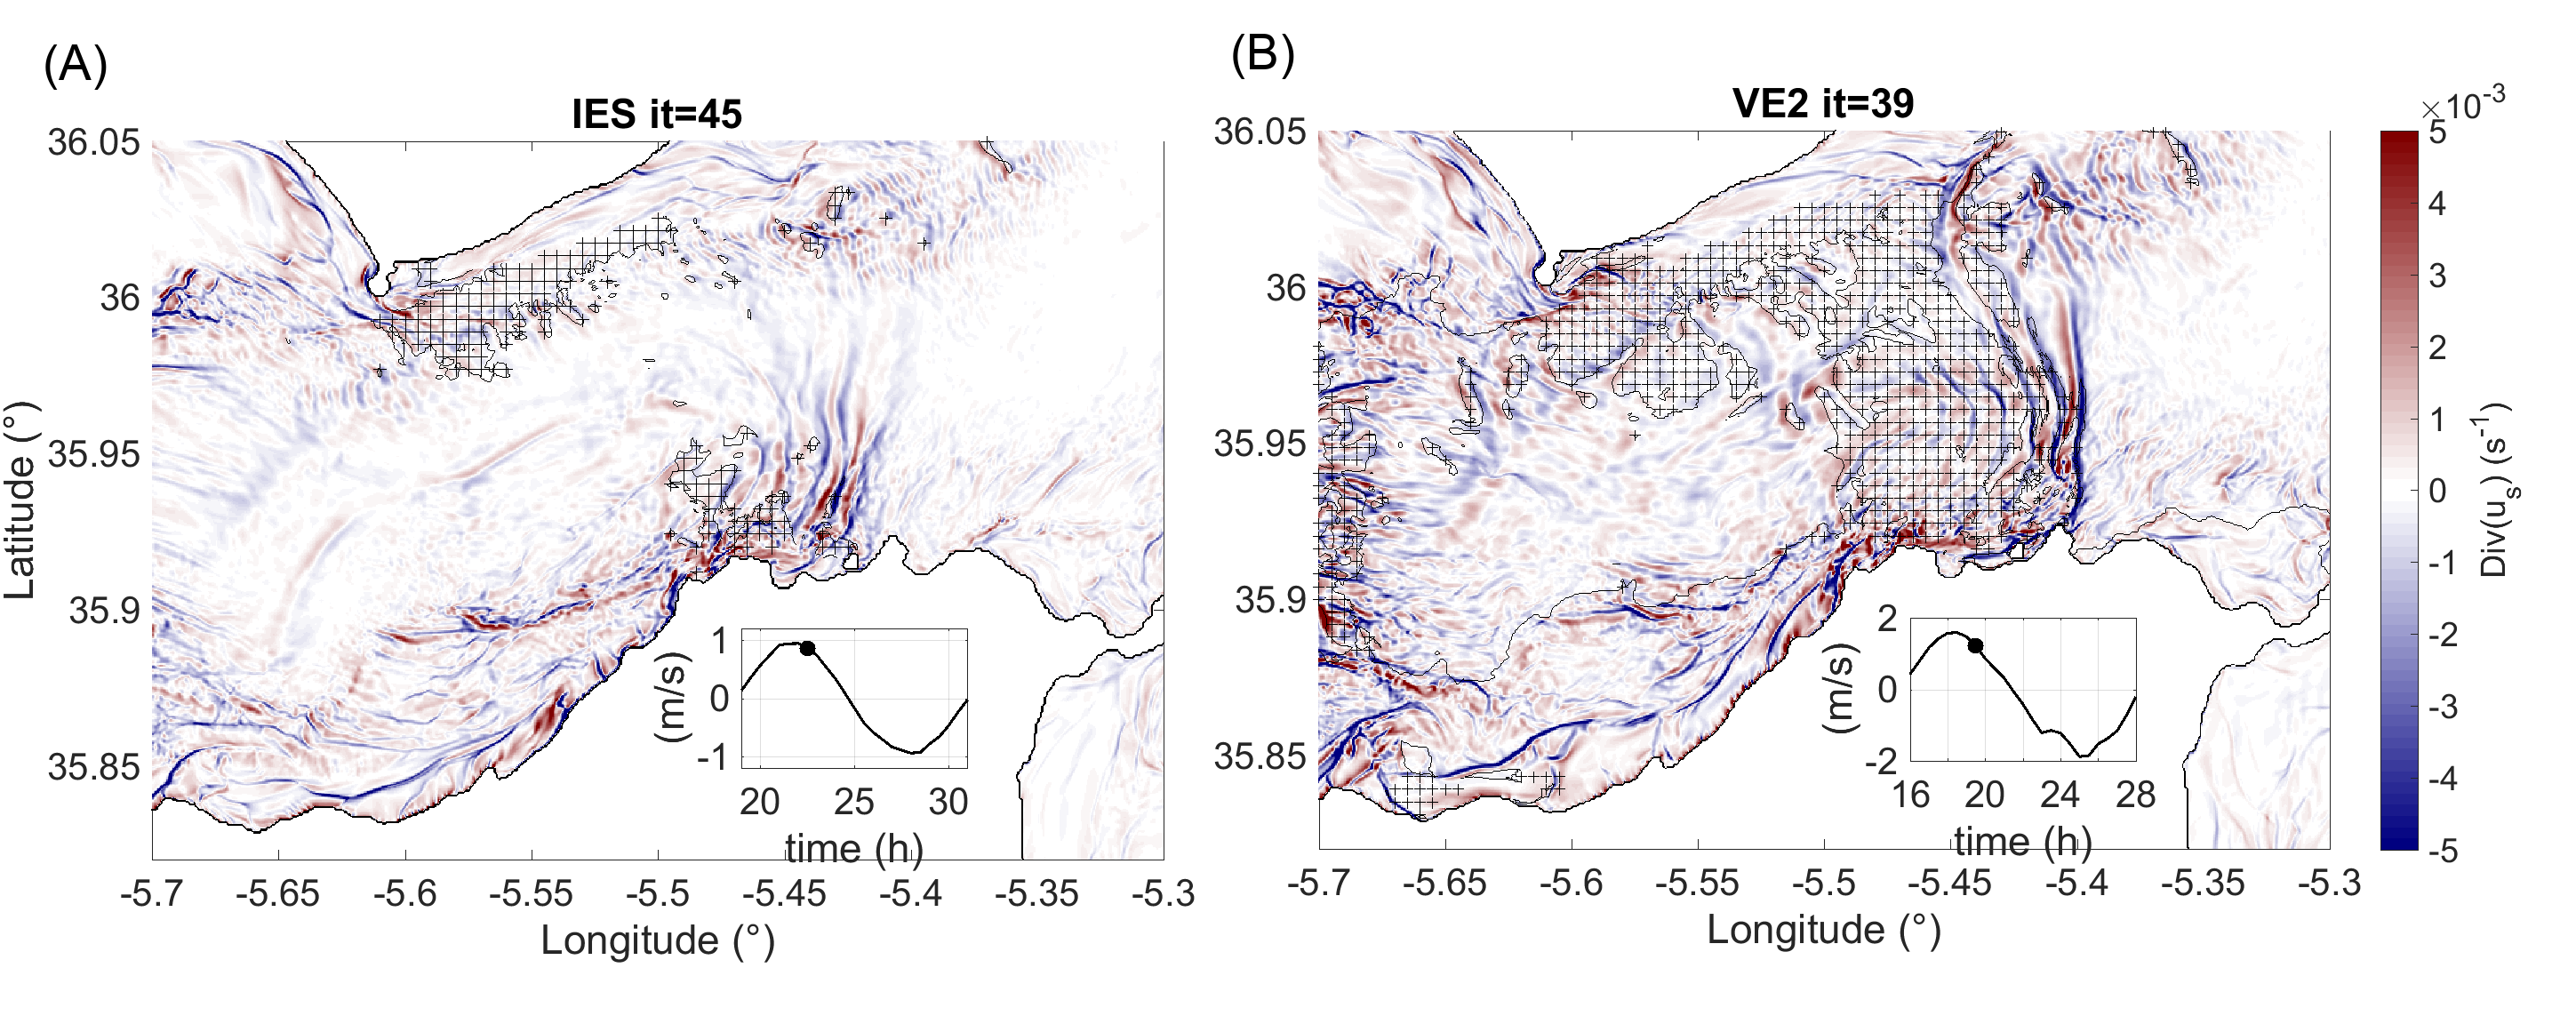
\includegraphics[width=\linewidth]{./GBR3D/FigWaveCont.png}
%\end{subfigure}
 \caption {Divergence of the surface current (color) and areas of supercritical Atlantic layer (black hatches) at t = 22.5 h in SimIT (A) and t = 19.5 h in SimST (B)}
 \label{FigISWGBR3D}
\end{figure}

\subsubsection{Propagation of Solitons (ISWs)}
\label{section_sim3D_ISW}

\begin{figure}[!h]
 \centering
 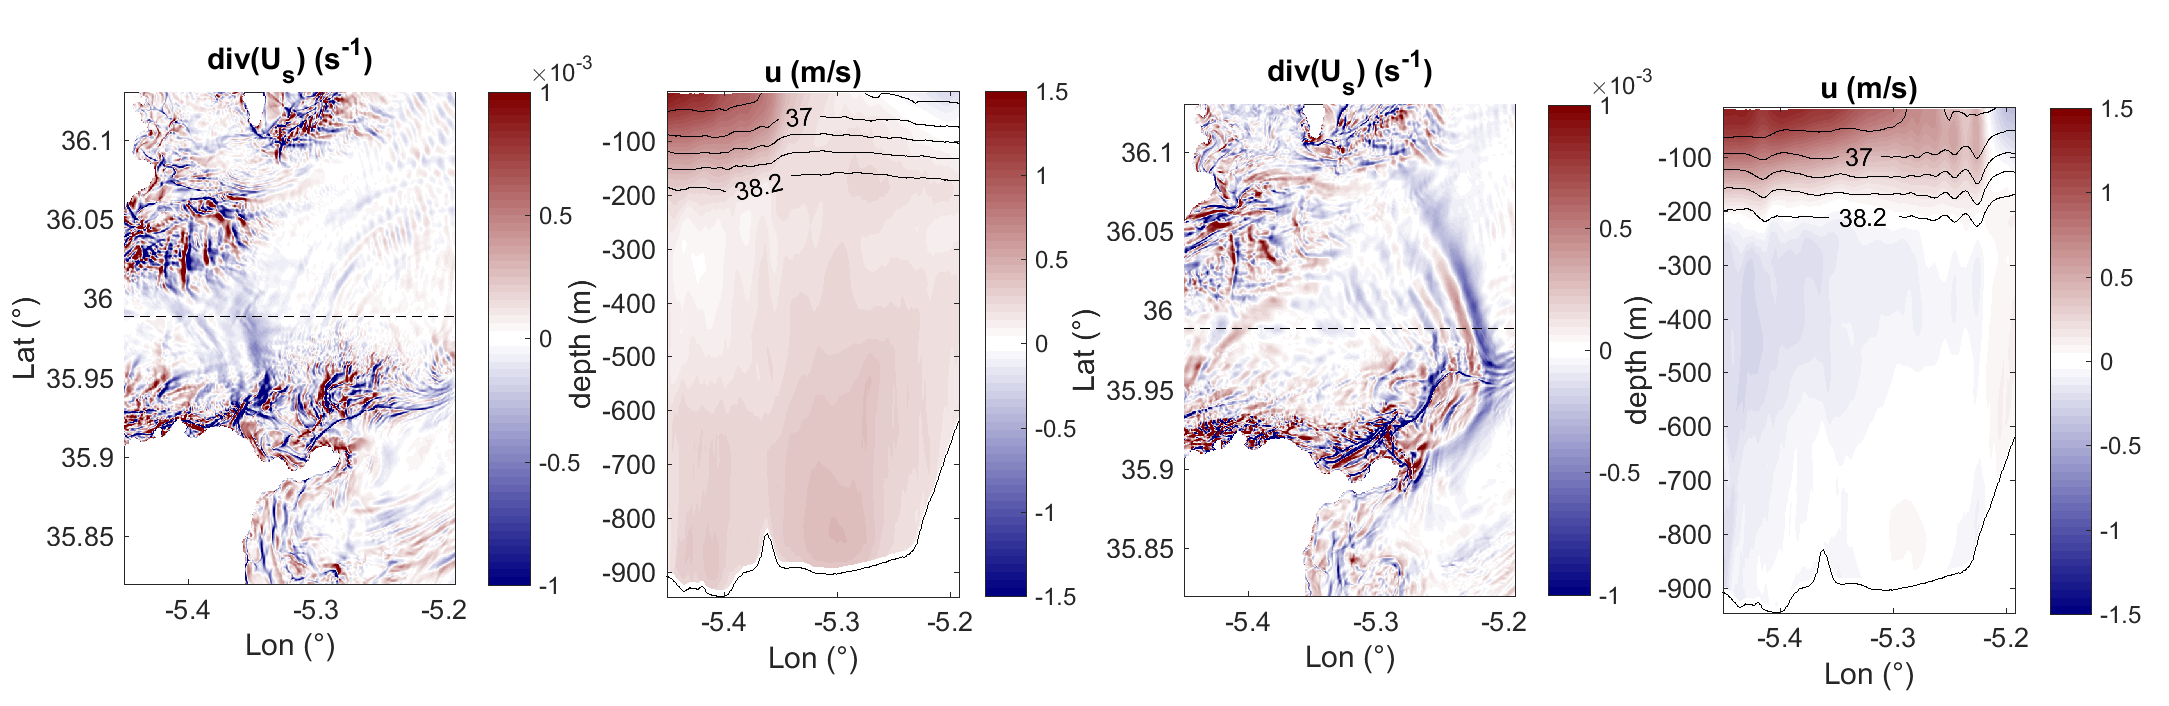
\includegraphics[width=1.\textwidth]{./GBR3D/coupesISW_ME2-2.png}
 \caption {Divergence of surface current (A1, A2) and vertical sections (B1, B2) of salinity (black isohalines) and zonal velocity $u$ (color) in SimNT at t = 20 h (A1,B1) and 22 h (A2,B2) of simulation.}
  \label{FigISWNT}
\end{figure}

\begin{figure}[!h]
 \centering
%\begin{subfigure}{\linewidth}
%\centering
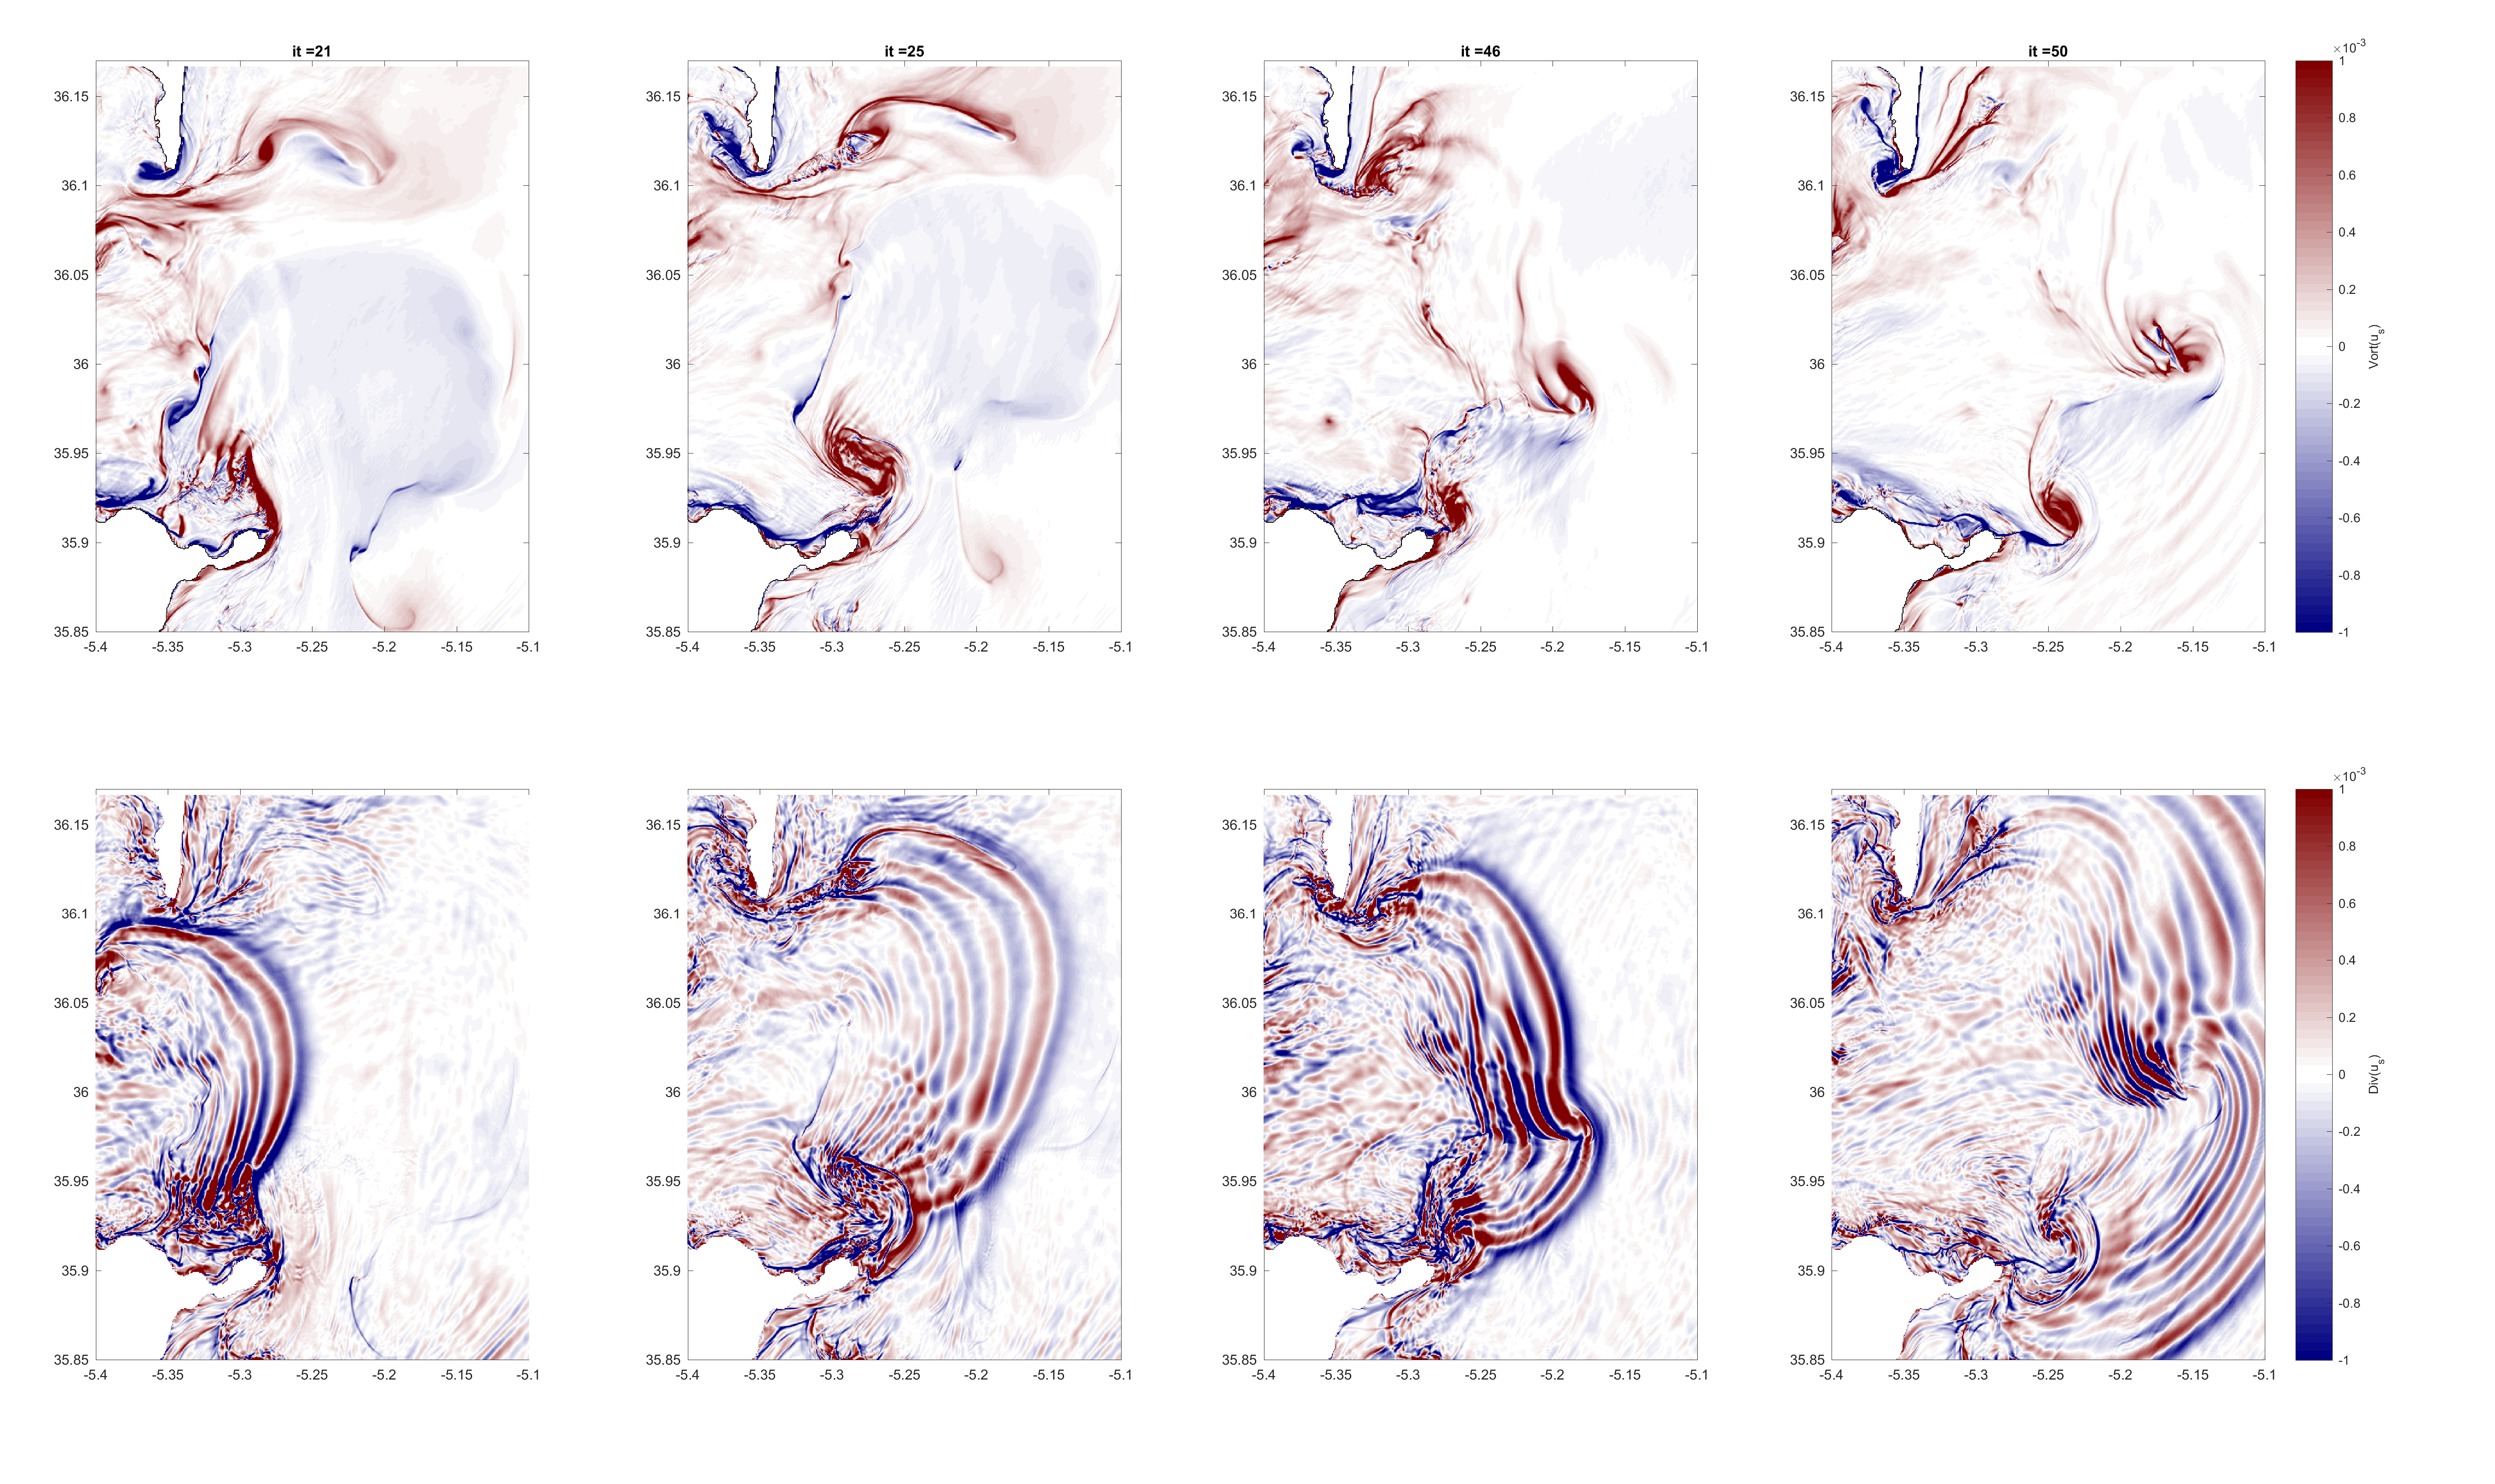
\includegraphics[width=\linewidth]{./GBR3D/FigTourbVE2.png}
%\end{subfigure}
 \caption {Divergence of surface current (upper row) at t = 10.5 h, 12.5 h, then 23 h and 25 h of simulation SimST, and z-axis vorticity of surface current (lower row) for the same instants.}
 \label{FigeddGBR3D}
\end{figure}

\subparagraph{Generation in \textit{no-jump} condition.}
Solitary waves are observed in the three simulations after the relaxation of the hydraulic jump at CS (figure \noparref{FigISWGBR3D}). Figures (\noparref{FigISWNT}.A1) and (A2) also depict the divergence of surface currents but at the eastern exit of the strait, at two consecutive times of an inflow following a no-jump outflow in simulation SimNT. Figures (\noparref{FigISWNT}.B1) and (B2) are vertical sections of the zonal current and salinity at the same dates. Despite taking place after a \textit{no-jump} outflow, a train of ISWs can be observed in figures (\noparref{FigISWNT}.A2) and (B2). This train, that ends up propagating in the Alboran sea, appears after the propagation of the baroclinic tide in figure (\noparref{FigISWNT}.B1) creates a growing front with isohalines steepening due to non-linear effects. As is the case for the ISWs generated at CS, non-hydrostatic dispersion balances this effect and creates a train of ISWs. In SimNT this process occurs following every \textit{no-jump} outflows.

However, compared to the upper row of figure \ref{FigeddGBR3D} (also showing the divergence of surface currents during two inflow periods following the presence of an hydraulic jump at CS), the train of ISWs visible at the surface in the Alboran Sea after a \textit{no-jump} outflow is less extended, consisting of fewer waves (3 in figure (\noparref{FigISWNT}.A2) and 5 in figure (\noparref{FigeddGBR3D}.A2)).

\subparagraph{Interaction with submesoscale eddies.}
Figures (\noparref{FigeddGBR3D}.A1) and (B1) then (\noparref{FigeddGBR3D}.C1) and (D1), show two consecutive inflow periods in the SimST configuration. The lower row of figure \ref{FigeddGBR3D} exhibits the z-component of the surface vorticity at the same time. In the first two figures of each row, a train of ISWs leaves the strait and enters into the Alboran sea. The number of solitons in the train increases during this period. A filament of positive vorticity is formed by interaction with the southern coast (Peninsula of Almina) in figure (\noparref{FigeddGBR3D}.A2) and develops into a cyclonic eddy in (\noparref{FigeddGBR3D}.B2). In figure (\noparref{FigeddGBR3D}.C2), one tidal cycle later, the eddy is located at 5.2 $^\text{o}$ W and 36$^\text{o}$ N and the new train of ISWs is refracted by this eddy in (\noparref{FigeddGBR3D}.C1) : its southern part is indeed accelerated whereas its northern part is decelerated by the induced currents. At the same time, a naw vortical structure can be observed off the southern shore. In figure (\noparref{FigeddGBR3D}.D2) this structure has also evolved into a cyclonic eddy, centered at 35.92°N;5.25°W, that propagates in the Alboran sea. Meanwhile, the interaction between the solitary waves and the previous cyclonic eddy has resulted into an interference pattern in the wave packet in figure (D1). 

In the simulations, this process of generation of cyclonic eddies in the peninsula of Almina occurs each time a train of solitary waves exits the strait. The train of the next tidal cycle gets diffracted on this eddy, creating local modifications of the structure of the train.

\subsubsection{Dynamical structures at Camarinal Sill, primary instabilities}
\label{sectionsim3D_res_insta}

\begin{figure}[!h]
% \centering
 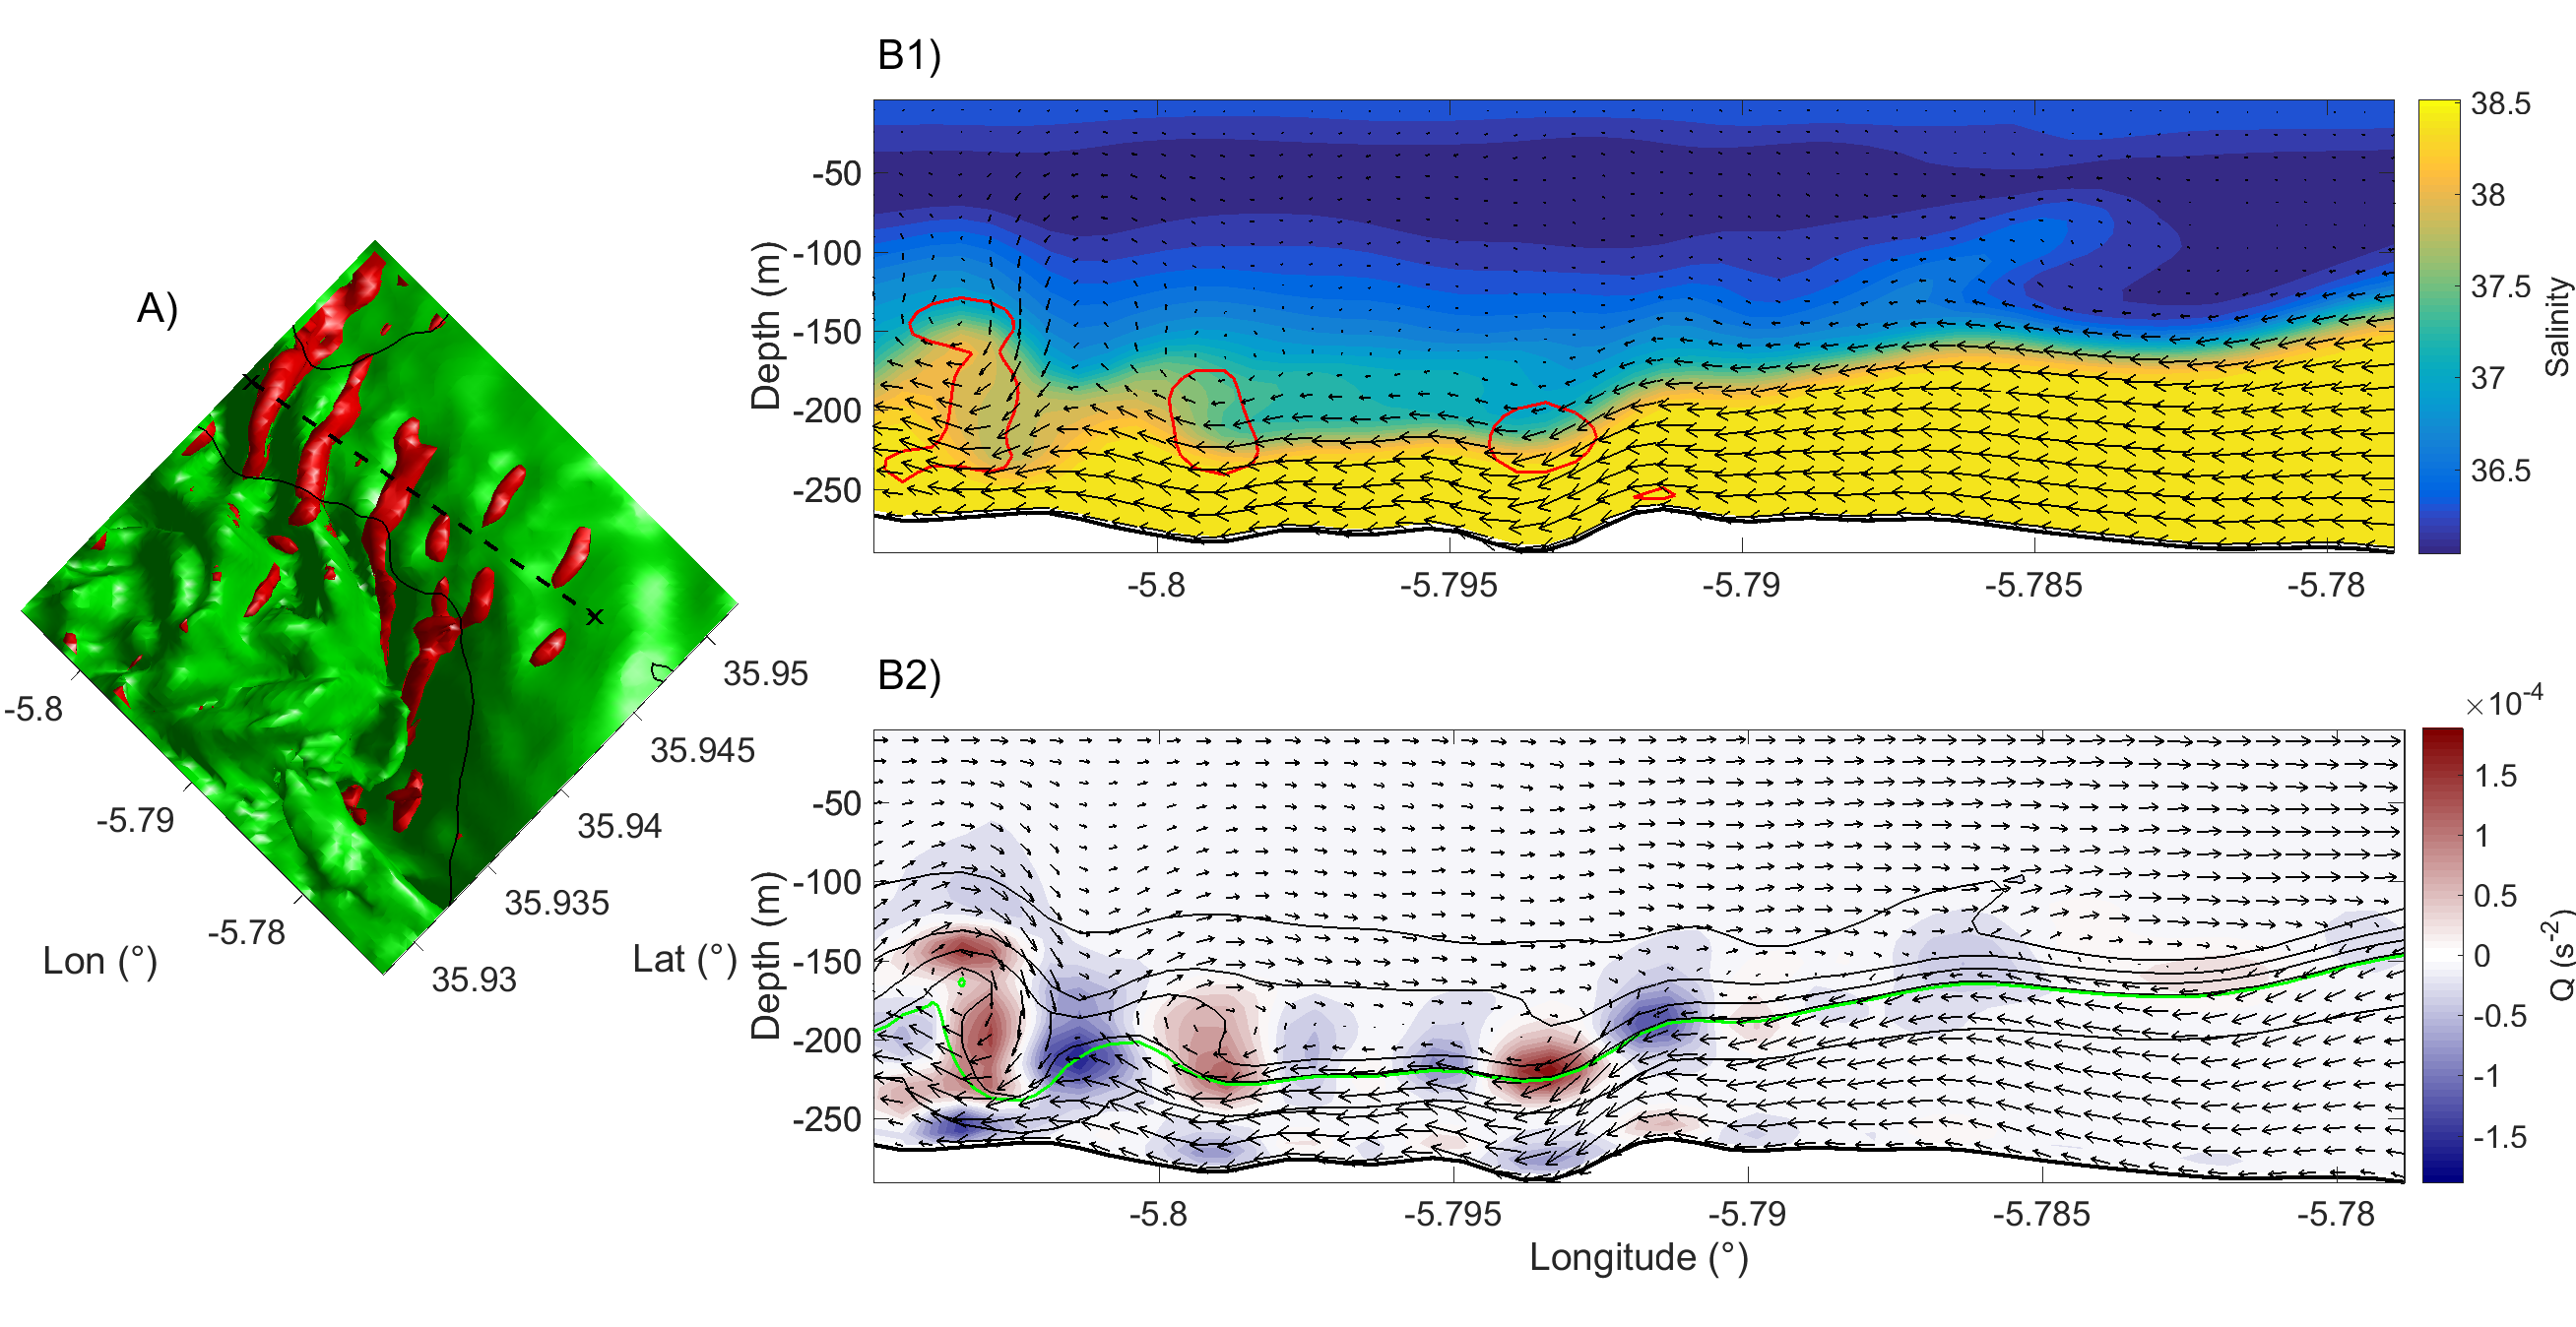
\includegraphics[width=\textwidth]{./GBR3D/FigInstaQ_IES4H.png}
 \caption {(A) Bird's eye view of isohaline surface $S=38.1$ (green) and $Q=5.10^{-5} \ s^{-2}$ surfaces (red) in a small area west of CS at t$=$4H in SimIT. 300-m depth isobath (black line) and position of the vertical section for B1 and B2 (dotted black line). (B1) Vertical section of salinity (color), ($u$,$w$) vectors and isoline $Q=5.10^{-5}\ s^{-2}$ (red). (B2) The same vertical section as (B1) with parameter $Q$ (color), isohalines (black lines and green line for $S=38.1$), and vectors ($u'$,$w$) where $u'$ is the residual of $u$ minus its barotropic component.}
 \label{FigInstaEx}
\end{figure}

\subparagraph{Standard deviation of paramater $Q$.}
Along with the features of the flow already discussed previously, figures \ref{FigHCN}, \ref{FigHCS} and \ref{FigHCI} indicate patches of high standard deviation of parameter $Q$ (defined in \S \ref{sectiondiagQ}). Figure \ref{FigInstaEx} gives an exemple of what the instantaneous field of $Q$ looks like in simulation SimIT. (\noparref{FigInstaEx}.A) presents a 3D bird's view of a serie of tube-like structures for which $Q=5.10^{-5} \ s^{-2}$ (in red) over a surface of constant salinity (in green). Those features are present in a small area immediately northwest of Camarinal Sill during an outflow and are moving westard. Figures (\noparref{FigInstaEx}.B1) and (B2) are vertical sections. (B1) shows the contour of $Q=5.10^{-5} \ s^{-2}$ (in red) along with the (u,w) component of velocity and the salinity in this section. In this velocity field, three areas of highly positive parameter $Q$ are positioned in the haloclyne between the Mediterranean and Atlantic waters.

In figure (\noparref{FigInstaEx}.B2), instead of (u,w) is plotted (u',w) with $u'=u-|u|$ where $|u|$ is the barotropic component of the zonal velocity. It highlights the area of shear between the Mediterranean vein and the Atlantic waters, but also confirms that the high positive values of $Q$ are associated with areas of rotating fluid, for exemple at 5.798°W and 200m deep. 

Those kind of structures are numerous and are carried westward by the Mediterranean outflow, meaning that over a single grid cell, the temporal evolution of $Q$ shows oscillations between high positive values (at the center of a billow or a vortex for instance) and low negative values (sheared layers between two consecutive billows for instance) as between the two westernmost vortexes of figure (\noparref{FigInstaEx}.B2). At such a grid point, the standard deviation of parameter $Q$ is large. Thus, this proxy is used in figures \ref{FigHCN}, \ref{FigHCS} and \ref{FigHCI}, where the maximal value of standard deviation in the water column is depicted. It indicates the areas where primary shear instabilities are advected by the Mediterranean Outflow. The higher the value of standard deviation is, the closer they are to the generation site.

\subparagraph{Neap-spring tide cycle in the Strait.}
Comparing the fields of standard deviation of $Q$ in figures \ref{FigHCN}, \ref{FigHCS} and \ref{FigHCI}, the extension of patches of standard deviation is maximal during all outflow periods, and the spring tide inflow of figure (\noparref{FigHCS}.A1) although the values of standard deviation for this latter case are not as large and the patch itself is not as extended. During the outflow cases, high values of standard deviation extend from the west of CS at 5.79 $^\text{o}$ W and west of secondary bathymetric features in Tangier basin at 5.84 $^\text{o}$ W. This values are higher for the two cases where an hydraulic jump is present at CS (\textit{s-jump} and \textit{w-jump}). There is also a smaller amplitude signal at ES.

More local patches exist east and west of CS, but with relatively small values of standard deviation that may not be associated with shear instabilities but with propagating internal gravity waves.


\subparagraph{Mixing along the path of the Mediterranean Outflow.}
Figure (\noparref{FigTSCS}.A) superposes the standard deviation of $Q$ and the singular vector of Singular Value Decomposition (SVD, see annexe \ref{annexeSVD}) performed on the 3D field of this same parameter $Q$ during an outflow of SimST. The singular vector depicted is the fifth one of the decomposition, the most high-ranked singular vector for which temporal evolution shows high frequency variability (timescale in minutes), associated with propagation of vortices (the higher ranked singular vectors (not shown) have low frequency variability and structure associated with the large-scale flow itself). Figures (\noparref{FigTSCS}.B1) to (\noparref{FigTSCS}.B4) are $\theta$-S diagram showing the signature of all the simulation grid-points at a given longitude, zoomed in on the domain of Mediterranean waters, at t$=$14h during this same outflow.

As expected, in figure (\noparref{FigTSCS}.A) the contours of parameter $Q= 5.10^{-5}\ m^2s^{-2}$ of the singular vector (in red) are colocalised with the highest values of sandard deviation of $Q$, i.e. on the western slope of CS (between 5.73°W and 5.8°W) and on the western slope of secondary sills in Tangier Basin (at around 5.84°W). At this latter location, three main areas appear for the generation and propagation of primary instabilities, from south to north : 35.88°N, 35.95°N and 36°N. Those are the same latitudes along which the Meditteranean water masses are homogeneizing in the $\theta$-S diagrams of figures (\noparref{FigTSCS}.B2) and (\noparref{FigTSCS}.B3). This is in accordance with previous results showing that the instabilities develop along the path the Mediterranean vein takes in the lee of bathymetric features. 

This orgaisation is absent in figure (\noparref{FigTSCS}.B1) for which at 5.76$^{\text{o}}$ W, still over the crest of Camarinal Sill, the composition of Mediterranean waters remains similar to the one found in figure \ref{Fig_Ini_WM3D} at the east entry of the strait.

The waters of the different Mediterranean vein's pathway are not homogeneous directly downflow of CS, highlighting how gradual the process of mixing is. While the primary instabilities are generated, diapycnal mixing itself, through the rest of the turvulent cascading process, has not yet occured entirely. It is in figures (\noparref{FigTSCS}.B3) and (\noparref{FigTSCS}.B4) that the Mediterranean veins are distinct and homogeneous, with the southern veins of the MEditerranean outflow being comprised of waters with higher density. In (\noparref{FigTSCS}.B4) the northernmost signal, of waters propagating  over 36°N, has been erroded and shows up outside of the zoomed aread of this figure in the $\theta$-S diagram. 

\begin{figure}[!h]
% \centering
 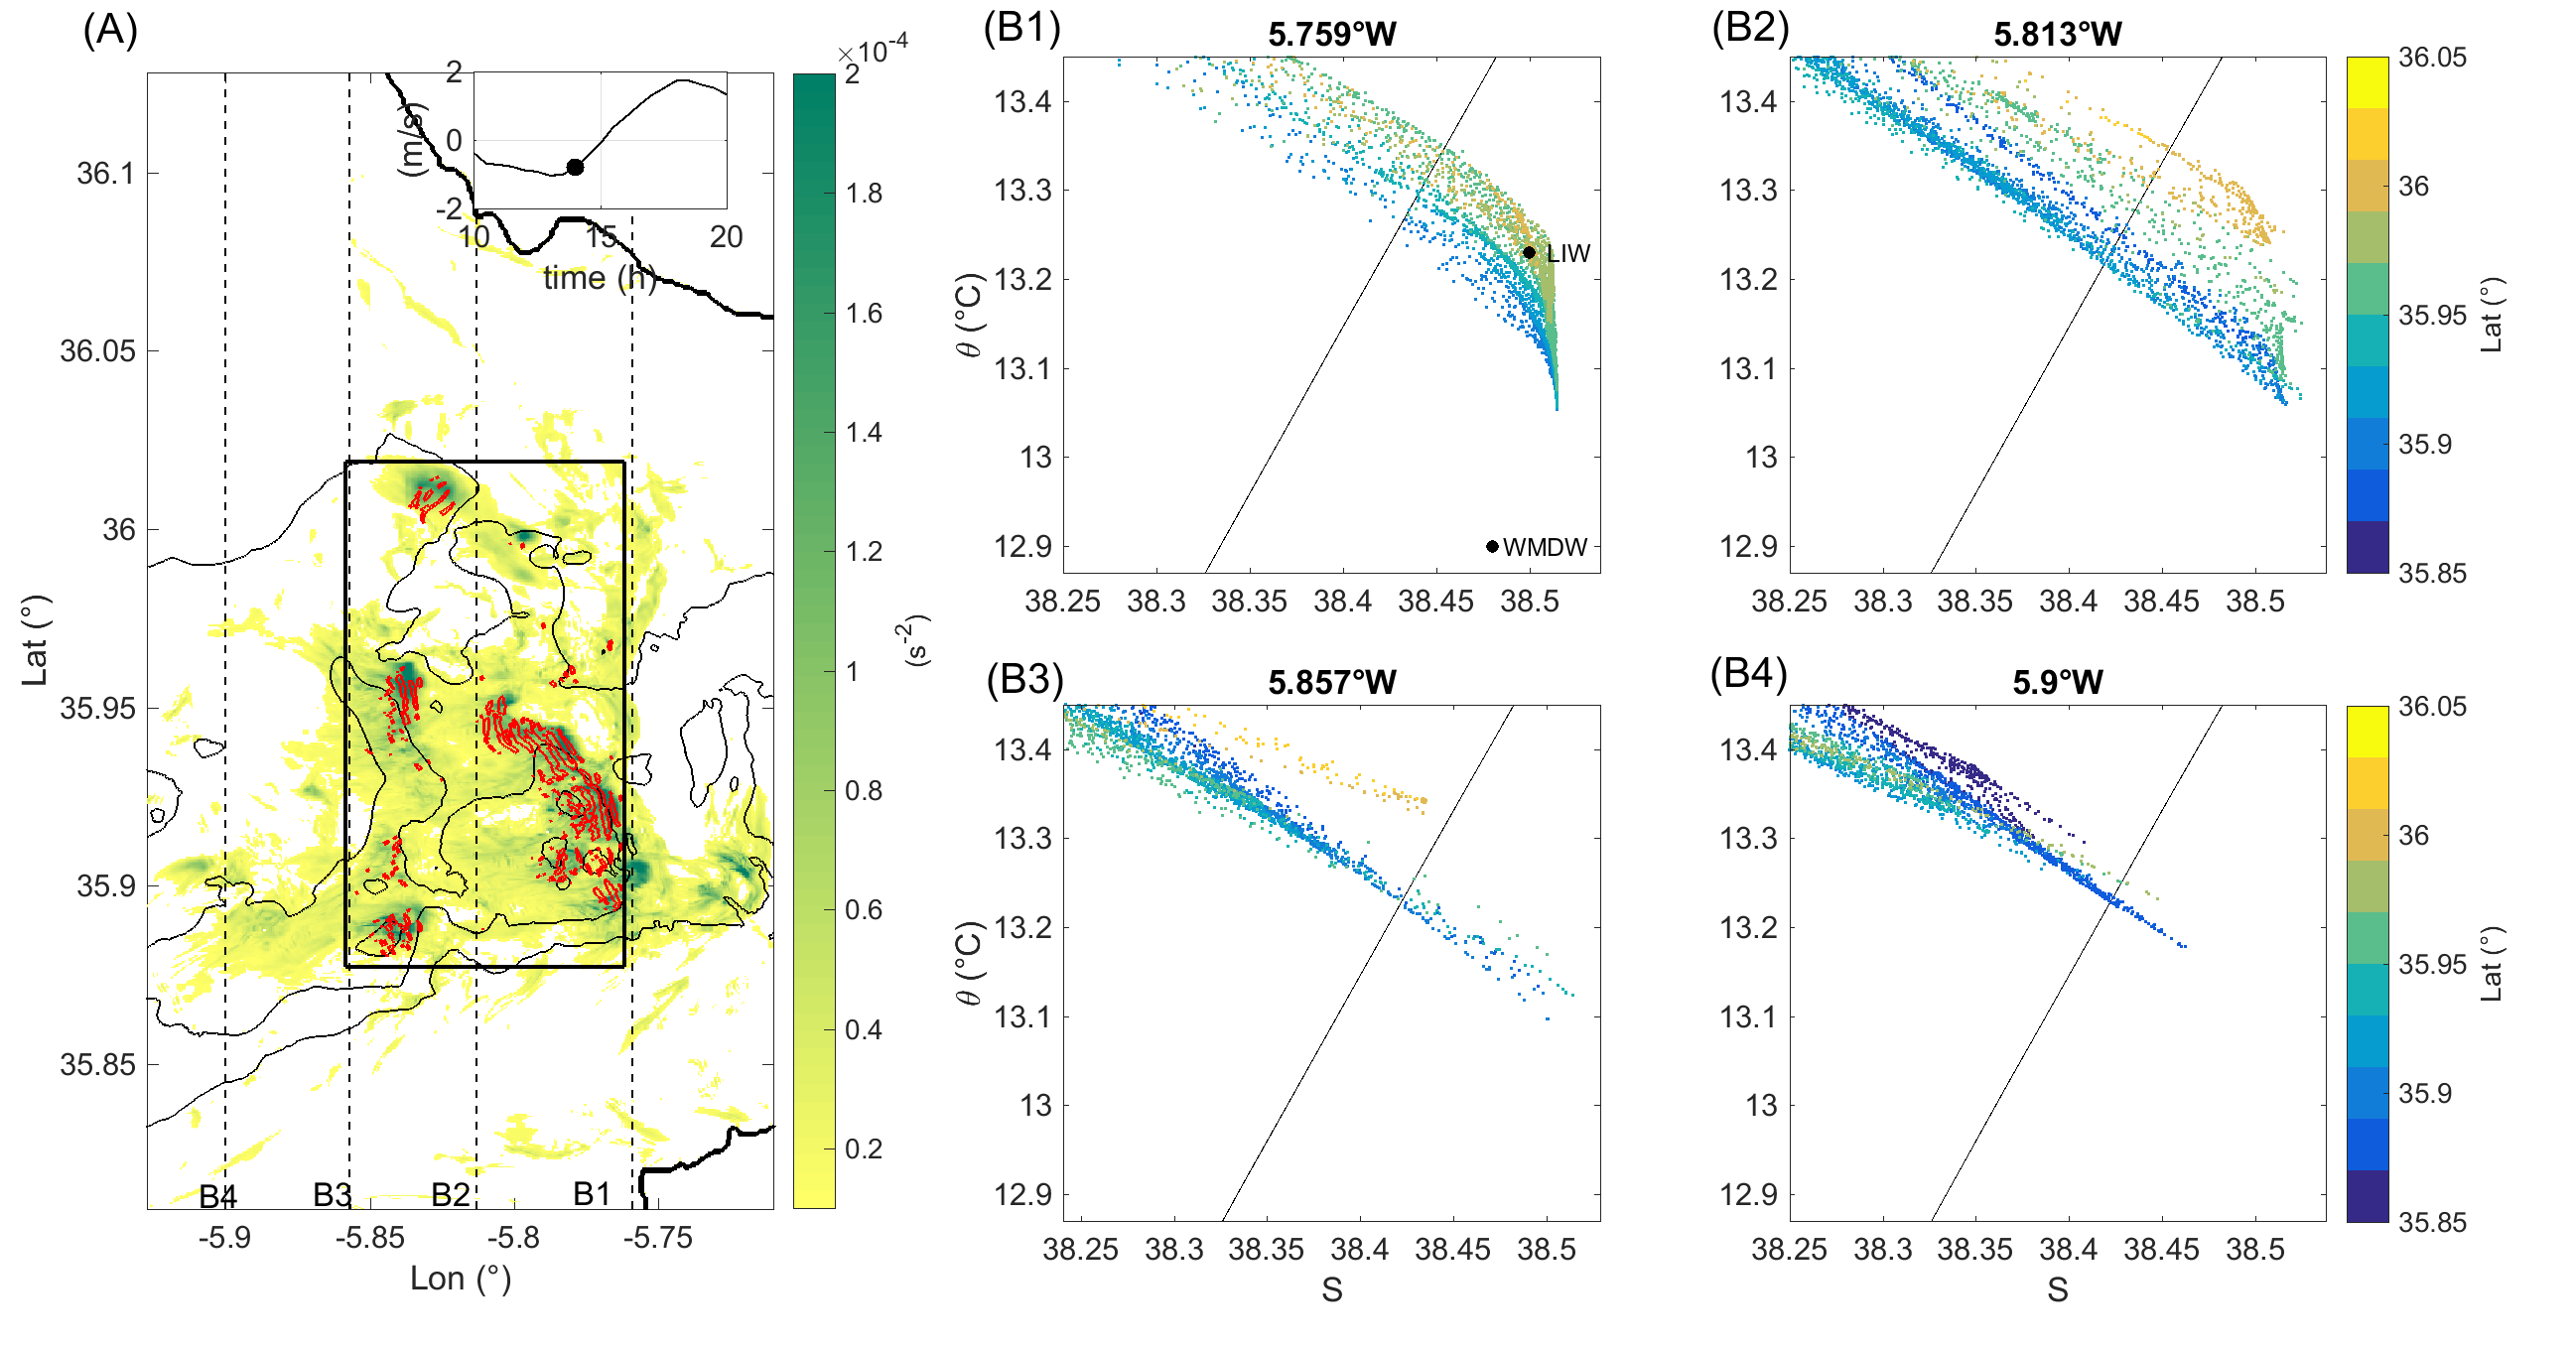
\includegraphics[width=\textwidth]{./GBR3D/TS_coupes_14H_VE2o.png}
 \caption {(a) Standard deviation of parameter Q over 30-mn-periods at $t\ =\ 14\ h$ in SimST (color) and isocontour of Q $\ =\ 5 s^{-2}$ from the high-frequency singular vector of SVD performed in the rectangular black box during the outflow period. Black dashed lines indicate the longitude at which $\theta-S$ diagrams are plotted. (B1, B2, B3, and B4) $\theta-S$ diagrams, zoomed in the area of the Mediterranean water masses, in color is the latitude of each point.}
 \label{FigTSCS}
\end{figure}

\subparagraph{Neap-spring tide cycle at CS.}
The singular vectors of SVD are now studied over outflows of simulations SimNT, SimIT and SimST, varying the strength of barotropic tidal currents, specifically over the area of Camarinal Sill. Figures (\noparref{FigEOFMIV}.A1, B1, C1) present the singular vector of parameter $Q$ for the outflows of figures \ref{FigHCN}, \ref{FigHCI},and \ref{FigHCS} respectively.

Along those, vertical sections of salinity are plotted in figures (\noparref{FigEOFMIV}A2,B2,C2). These sections are plotted along latitude 35.94$^\text{o}$ N. Figure (\noparref{FigEOFMIV}.D) and (\noparref{FigEOFMIV}.E) are histograms giving the height above the seafloor and the latitude of the grid points of the singular vectors of figures (A1,B1,C1) for which $Q$ is larger or equal to $5.10^{-5}\ s^{-2}$. On vertical sections, positive values of $Q$ parameter are associated with specific billow structures of salinity that develop in the gravity current along the west slope of the CS, as was the case in figure \ref{FigInstaEx}. 

Those structures are generated for each outflow case at a depth of around 100m above the seafloor for both hydraulic jump cases, and 70m above the seafloor for the no-jump case (figure (\noparref{FigEOFMIV}.D)). Instabilities are also more numerous for the w-jump outflow case in SimST (figure C1), developping along all latitudes as seen in figure (\noparref{FigEOFMIV}.E). Whereas, in the other two cases instabilities are not present between the interval of 35.925°N and 35.932°N west of the shallowest part of CS.

Looking at the vertical section of figure (C2), in the w-jump case the interface drop of the western hydraulic jump of CS is over the western slope at 5.775°W, contrary to figure (B2) of the s-jump outflow type for wich it is positioned at 5.755°W. In that s-jump case as well as the no-jump case of figure (A2), the dynamic over the slope is of a density current. In the w-jump case, this density current of Mediterranean waters overcoming the sill is colocalised with the hydraulic jump, including west of the shallowest point of CS. Only when the hydraulic jump is localised there can the Mediterranean waters flow over this shallow depth as the rapid Mediterranean vein in which primary shear instabilities can develop. 

In the vertical sections (B2) and (C2) the aspect the salinity billows structured by this instabilities is similar, with the core of the billows having low salinity that can reach 37 psu compared to the ambiant waters around 38 psu. Note that as this longitude, corresponding to the area of the $\theta$-S diagram of figure (\noparref{FigTSCS}.B2), the outflow is still heterogeneous. The aspect of the billows in the no-jump case of figure (\noparref{FigEOFMIV}.A2) is different and does not incorporate as much low salinity waters.


\begin{figure}[!h]
% \centering
 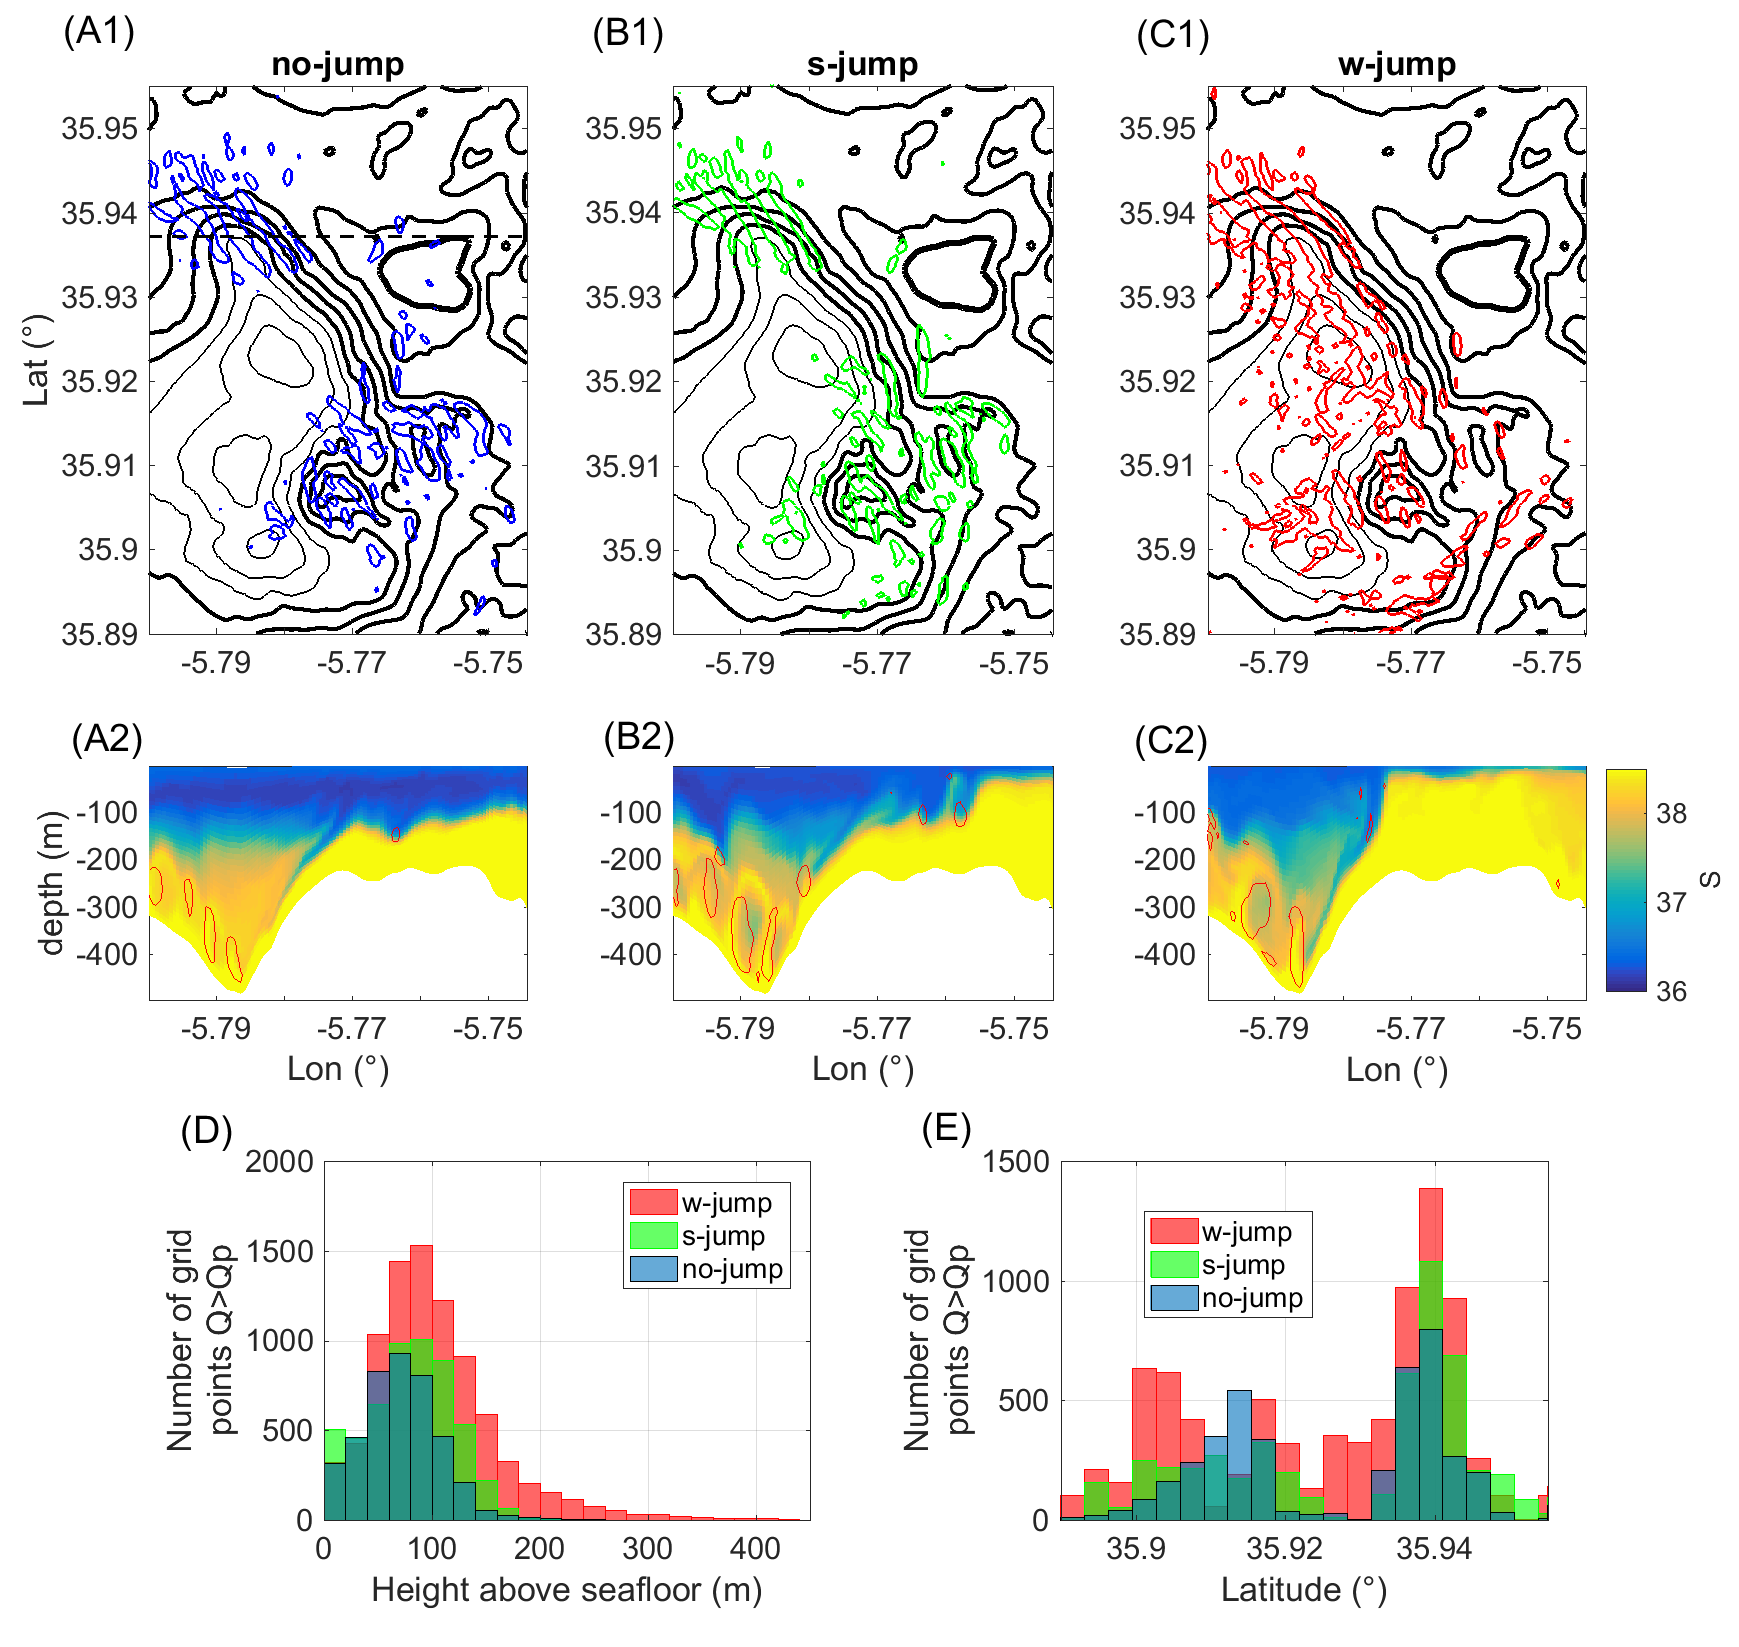
\includegraphics[width=\textwidth]{./GBR3D/EOF5_MIV_2D.png}
 \caption {(A1, B1, C1) Contours of parameter Q$\ =\ 5.10^{-5} \ s^{-2}$ in the first high-frequency singular vector of SVD performed during outflow of figures (\noparref{FigHCN}.A2),\ref{FigHCI} and (\noparref{FigHCS}.A2) respectively. Isobathes in black: 200 m (thicker), 250 to 450 m (thick) and 500 to 600 m (thin). (A2, B2, C2) Vertical sections of salinity (color) and contours of Q-parameter $\ =\ 5.10^{-5}\ s^{-2}$ at latitude $35.9372^\text{o}$ N at the same dates. (D) histogram of the height of the grid points of each singular vector shown in A1, B1 and C1 above the seafloor. (E) Same as (D) but showing the latitude of the grid points.}
 \label{FigEOFMIV}
\end{figure}

\subparagraph{Closure schemes.}

Four additional simulations are now presented to investigate and better understand the impact of the turbulent scheme: the first three are based on a different implementation of the Smakorinsky turbulent scheme and the latest uses the GLS K-$\epsilon$ scheme (see table \ref{tab_sim3Dnames}). 
In figure \noparref{Fig3Dsch}.A1, A2, A3 and A4), vertical sections of salinity during the first outflow after $t\ =\ 5\ h$ of a \textit{no-jump} outflow case. Values are indicated for the Richardson gradient number $Ri=0.25$ (black) and $Q =\ 5.10^{-5} \ s^{-2}$ (red). $Ri$ is calculated from fields of density and velocity averaged over half and hour to filter out the propagating structures.

Figures (\noparref{Fig3Dsch}.B1, B2, B3, and B4) show the salinity averaged in the Mediterranean (B1, B3) and Atlantic (B2, B4) layers as defined in \S \ref{sectiondiagControl}, west (B1,B2) and east (B3,B4) of CS. Keep in mind that averaged values are shown, and that as previously discussed and shown in figure \ref{FigTSCS}, at this longitude west of CS, the different veins of the Mediterranean outflow are not yet distinct. Primary shear instabilities carry waters of lesser salinity into the outflow, but it has not yet been homogeneized by further mixing processes.

The decrease in salinity of the layer this provokes depends of the turbulent closure scheme, but in a counterintuitive way. Looking first at averaged layer salinities east of the sill in figures (\noparref{Fig3Dsch}.B3 and B4), simulations SimIT-S001, SimIT-S01 and SimIT-Kep lead to the same salinities for the Mediterranean layer, whereas differences can be observed punctually in the Atlantic layer. The simulation presenting the largest differences is SimIT-S1: the Mediterranean layer is less saltier by 0.4psu after t$=$2h, whereas the Atlantic layer is, in contrast, saltier by 0.5psu compared to the other simulations. This is expected since in SimIT-S1, the mixing coefficient is larger, hence there is more diffusion accross the interface between Atlantic and Mediterranean waters.

However west of the sill in SimIT-S1, both the Atlantic and Mediterranean layers are saltier than in the three other simulations, especially between 2 and 8 hours following the initialization. This cannot obviously be explained by an increase of the dissipation that would lead to a salinity of the Meditteranean layer lesser than in the other simulations, the same way than it does in the eastern section.

At 5 hours of simulation, the vertical sections of figures (\noparref{Fig3Dsch}.A1,A2,A3 and A4) show that instabilities develop. The area where $Ri$ is lower than $0.25$ begins at 5.77$^\text{o}$ W in all the simulations, indicating shear instabilities could develop from this point in the gravity current. This is the case for SimIT-S01, SimIT-S001 and SimIT-Kep, but instabilities are only found downslope of an intrusion of Atlantic waters at 5.783$^\text{o}$ W in simulation SimIT-S1 (figure (A3)).

In simulations SimIT-S001 and SimIT-S01 (figures (A1) and (A2)), instabilities arise earlier in the hydraulic jump, which makes it that the waters at the center of the billows for exemple at 5.778°W are of small salinity and originate in the Atlantic layer, whereas in SimIT-S1 the billows are forming incorporating ambiant mixed waters of the Mediterranean vein to the new saltier Mediterranean waters that cross the sill. In SimIT-S1, less Atlantic water is integrated to the Mediterranean outflow when going through CS, resulting inf figure (\noparref{Fig3Dsch}.B1) to a saltier Mediterranean layer than in the other three simulations.
 
In the case of implementation of $K-\epsilon$ turbulent scheme in simulation SimIT-Kep, the billows, and more generally the instabilities, are less-developped with smaller values of parameter Q in figure (A4) and a less-salty outflow in (B1). This signal persists $7\ h$ after the initialization when the flow reverses and no instabilities are generated anymore accross all simulations. For SimIT-S1, at this point the salinity averaged in the MEditerranean layer is closer to the other simulations with Smagorinsky schemes, possibly because the increased diffusion in the pycnocline may counteract the previous enhanced injection of Mediterranean water.

\begin{figure}[!h]
% \centering
 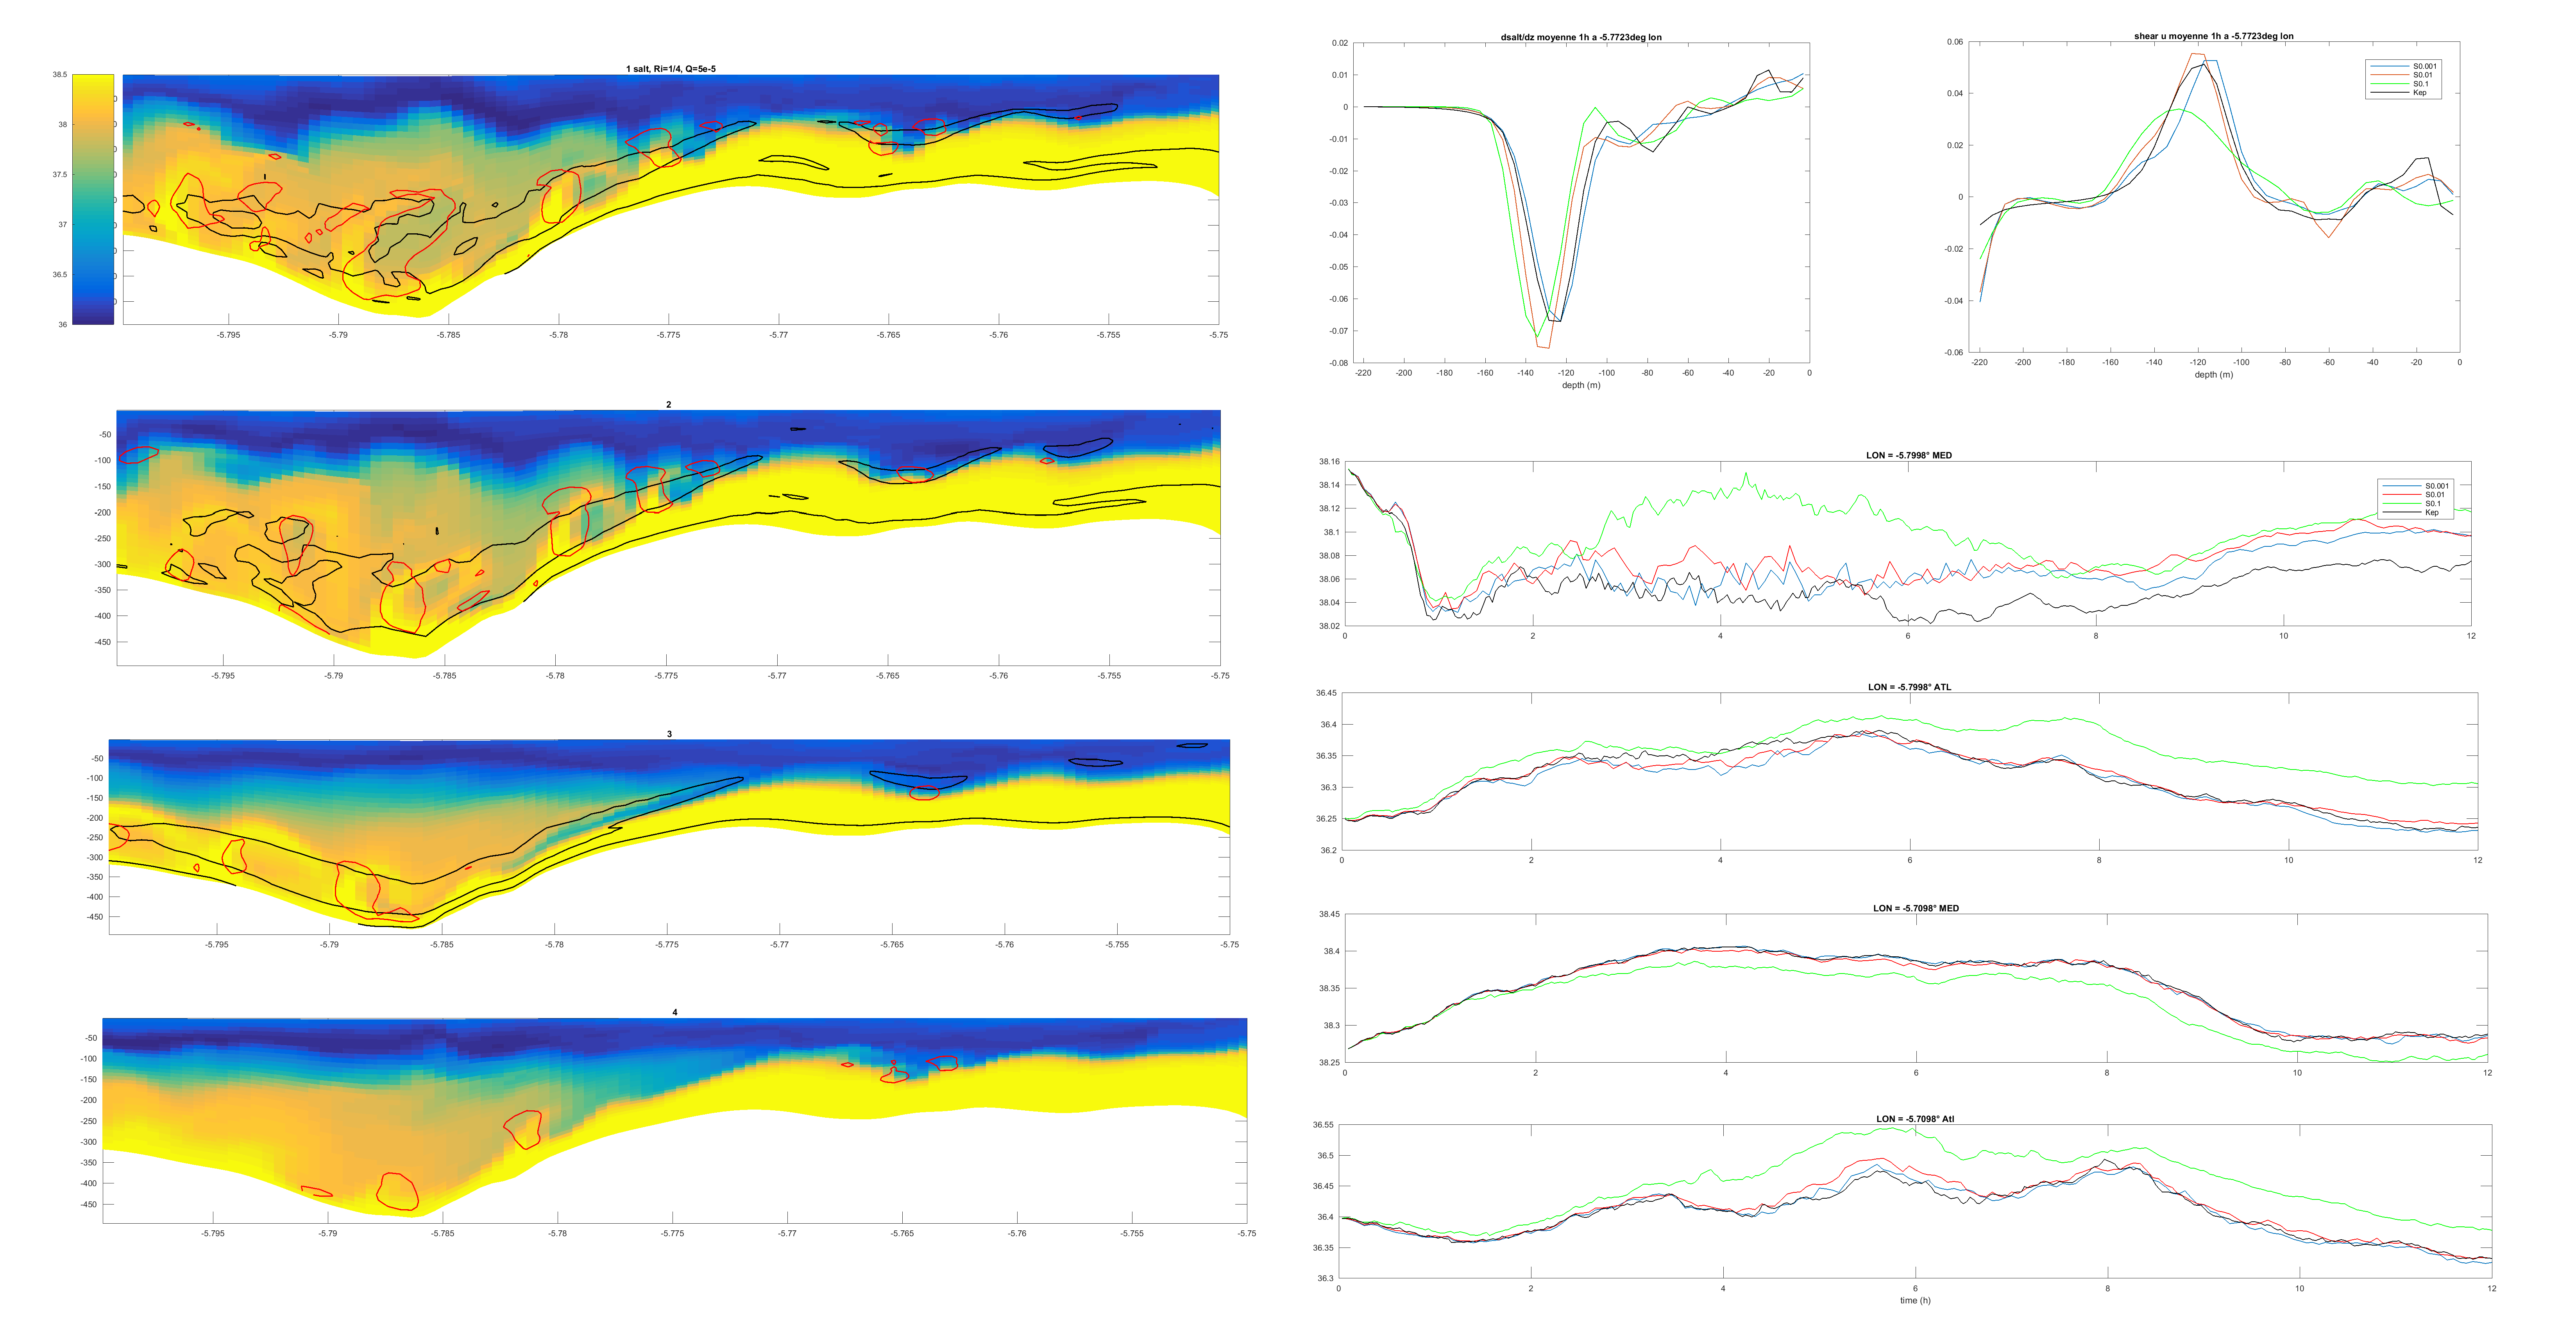
\includegraphics[width=\textwidth]{./GBR3D/Figsmago.png}
 \caption { (A1, A2, A3, A4) Vertical section of salinity (color), contours of $Q = 5.10^{-5} \ s^{-2}$ (red) and Richardson gradient number $=\ 0.25$ (black) at a latitude of $35.9372^o\ N$ in SimIT-S001, SimIT-S01, SimIT-S1 and SimIT-Kep IES respectively, 4 h after the initialization. (B1,B2,B3 and B4) Averaged salinity accross the Mediterranean or Atlantic layer at two different longitudes.\color{red}(Mettre lettres et bons noms de simus)\color{black}}
 \label{Fig3Dsch}
\end{figure}

%----------------------------------------------------------------------
\subsection{Discussion \& conclusions}
%----------------------------------------------------------------------
\subsubsection{Fines scales in Gibraltar strait.}
The variability of the hydraulic control and the variability of the other dynamical features during the neap-spring tidal cycle have been explored with high resolution, non-hydrostatic, free-surface simulations of the region of the Gibraltar strait. No permanent supercritical flow has been identified in the various simulations and only intermittent events of such flows have been observed during the tidal cycle. The location and the extension of the area of supercritical flows depend on the strength of the barotropic currents. During tidal outflows when both Atlantic and Mediterranean layers are critical at Camarinal Sill, two hydraulic jumps are generated and explicitly simulated. The western one is located either over the shallowest part of the sill (\textit{s-jump} case), or over its western slope (\textit{w-jump} case). 

For the western jump, this displacement during spring tide is similar to the behaviour that was simulated by \citet{sanchez-garrido_2011}. However, these authors found that for this tidal forcing the eastern hydraulic jump was also swept on the western slope of CS, while in our case this eastern hydraulic jump, while being swept westward, remains close to its initial position east of the sill, and is still a distinct hydraulic jump. This discrepancy seems to arise mainly from differences in bathymetric data between the two models: the eastern bathymetric feature is not as prominent in \citet{sanchez-garrido_2011} as in the present study.

A secondary generation process for ISWs has also been brought to light. To our knowledge, previous studies focused so far exclusively on the generation of ISWs following the collapse of the hydraulic control at "high tide" in the region of the strait. During tidal cycles with no critical flow over the sill and no hydraulic jump, the propagation of a long internal wave induces, through non-linear steepening of the wave and non-hydrostatic dispersion, the generation of a smaller (less extended) train of ISWs in the eastern part of the strait.

During each simulated tidal cycle, a cyclonic eddy is formed along the coast of the Peninsula of Almina (southern part of the eastern exit of the strait of Gibraltar). This eddy is advected by the flow in the Alboran sea and interacts with the trains of ISWs, inducing a local diffraction of the solitons. 

Several other dynamical features have been explicitly simulated such as the billows resulting from shear instabilities and developing in the lee of CS. In simulations, these billows are associated with high positive values of parameter $Q$. This parameter is used as a proxy for their detection and analysis. The billows are generated at the interface of Mediterranean and Atlantic waters and they are advected by the Mediterranean outflow while carrying waters of lesser density originating from the interface or the Atlantic layer. They are also present above secondary bathymetry accidents in Tangier basin and above ES. They can be observed during outflows of any intensity, but their spreading changes with the intensity of tidal currents, due to the existence and to the position of the western hydraulic jump at CS. They play an important role in the way the simulated Mediterranean and Atlantic waters mix, changing the hydrological features of the Mediterranean vein. In numerical simulations, this mixing is sensitive to the dynamic of the instabilities, and this dynamic is piloted by the turbulent dissipation scheme.

A conclusion is that the hydrological and dynamical properties of the Mediterranean waters entering in the northern Atlantic basin are greatly influenced by the configuration of the flow in the region of CS. Both the volume of these Mediterranean waters and their mixing with the Atlantic waters can indeed vary during the neap-tide cycle. 

In the present numerical configurations, only the largest primary instabilities and thus only the upper part of the direct turbulent cascade were explicitly simulated. The route to mixing consequently depends on the quality of the turbulence closure scheme used to end up mixing the water masses and this dependency has been evaluated by testing several schemes with well-known properties. 

No atmospheric forcing were specified at the surface of the ocean in the configurations presented in this section. This means that the upper layer is not realistically represented in particular in the region of Tarifa Narrows where wind stress is expected to be the largest. This choice remains yet consistent with the desire to simplify (but not over simplify) the "fine" dynamical structures in the complex region of the strait of Gibraltar. But if taken into account, atmospheric forcing could inhibit the secondary generation of ISWs after no-jump outflow at CS that occurs repeatedly in simulations. Other processes could be affected by the absence of atmospheric forcing, like the formation of eddies at the exit of the strait and their advection into the Alboran sea that is probably influenced by the WAG.

\subsubsection{LES in the Strait of Gibraltar.}
To our knowledge, the present study is the first 3D Large Eddy Simulation in the region of Gibraltar strait. However, only primary instabilities developing at the interface between Mediterranean and Atlantic water masses have been explicitly simulated. Other primary instabilities  with length scales of a few meters or less can be expected in the surface and bottom layers. Such dynamical structures remain implicit and are modelized as subgrid processes with the 45m-resolution grid used in the present numerical configurations.

As a consequence the numerical configurations of this study can be  classified as Large Eddy Simulation of the inner water column, for which a resolution of a few tenths of meters both in the horizontal and vertical directions is sufficient in Gibraltar strait for to simulate explicitly primary instabilities.

In the real ocean, such primary instabilities devolve into secondary (then tertiary, etc.) instabilities that break there structure in various ways \citep{mashayek_2012}. How fast the transition between primary and secondary instabilities occurs will command the characteristics of the water masses in the Strait of Gibraltar. Since secondary instabilities do not occur with a still too coarse grid, the evolution of this instabilities is unnatural.

Moreover, the tools employed here to examine the rise of those instabilities in LES are limited and somewhat rudimentary in reflecting the stochastical nature of the turbulent process. It as been shown that the choice of subgrid dissipation parametrization generaly influences the primary instabilities dynamics, and it is crucial to develop accurate, dedicated tools to evaluate the diapycnal mixing provoked by those structures. Investigation of such a tool makes up the last chapter (chapter \ref{chapBPE}) of the present manuscript.

Finally, compared to the kilometric horizontal-grid length-scales classically proposed, the much higher resolutions proposed here obviously lead to an increase of the computer coast to cover the region of the strait. This could be achieved thanks to the performances of the CROCO model inherited in part from ROMS time-splitting and numerical schemes \citep{shchepetkin_regional_2005} in which a non-hydrostatic, compressible kernel has been added \citep{auclair_non-hydrostatic_2018, hilt_numerical_2020}. This study is consequently a first step toward a downscaled, embedded, explicit simulation of the large turbulent structures when and where scale cascading leads to mixing in the water column.

The present work is thus a first LES exploration in \textit{Terra Incognita} \citep{scotti_large_2010, wyngaard_toward_2004}.\color{black}
\color{black}
